\documentclass[
	aspectratio=169,
	xetex,
	%notes,
]{beamer}
%\usepackage{pgfpages}
%\setbeameroption{show notes}
%\setbeameroption{show notes on second screen=bottom}
\usepackage{pdfcomment}
\usepackage{pdfpages}

\usetheme[
	%titleformat=smallcaps,
	background=dark,
	progressbar=frametitle,
	numbering=none,
]{metropolis}
\usecolortheme{owl}

\usepackage{appendixnumberbeamer}

\usepackage{booktabs}
\usepackage[scale=2]{ccicons}

\usepackage{pgfplots}
\usepgfplotslibrary{dateplot}
\usepackage[]{graphicx}
\usepackage[]{url}
%\usepackage[utf8]{inputenc} % only needed if not using xetex
\usepackage[]{hyperref}
\usepackage[english]{babel}

\usepackage{forloop}
\newcounter{i}
\newcounter{messagepages}

\newcommand*{\numberofpages}[1]{%
  \the\XeTeXpdfpagecount"#1" %
}
\setcounter{messagepages}{\numberofpages{out/messages.pdf}}
\stepcounter{messagepages}

%-----8<------------8<------------8<------------8<------------8<------------8<------------

\newfontfamily\fontfoundation[
    Path=fonts/
]{foundation-icons.ttf}
\newlength\fsize
\newcommand*\icon[3]{{
	\setlength\fsize{#2pt}%
	\fontsize{\fsize}{#3\fsize}\fontfoundation{#1}
}}

\newcommand\icontwitter[2][1.2]{\icon{}{#2}{#1}}
\newcommand\iconmail[2][1.2]{\icon{}{#2}{#1}}

%-----8<------------8<------------8<------------8<------------8<------------8<------------

%% When using Metropolis
%\setbeamercolor{frametitle}{%
%	fg=black!2,
%	bg=mDarkTeal
%}

%-----8<------------8<------------8<------------8<------------8<------------8<------------

\title{A look into the Mobile Messaging Black Box}
\subtitle{\scriptsize{33$^{\mathsf{rd}}$ Chaos Commmunication Congress \#33c3}}
\date{\today}
\author{
	\parbox[t]{1.2in}{Roland Schilling}{\scriptsize{\ttfamily @NerdingByDoing}}\\
	\parbox[t]{1.2in}{Frieder Steinmetz}{\scriptsize{\ttfamily @twillnix}}
}

\makeatletter
\hypersetup{
	pdfauthor=Roland Schilling \& Frieder Steinmetz,
    pdftitle={\@title},
    pdfsubject={Mobile Instant Messaging},
    pdfkeywords={Signal} {Threema} {33c3} {messaging} {reverse-engineering},
}\makeatother

\institute{Hamburg University of Technology\\
Security in Distributed Applications}
% \titlegraphic{\hfill\includegraphics[height=1.5cm]{logo.pdf}}


%-----8<------------8<------------8<------------8<------------8<------------8<------------

% stuff for arbitrary image placement
% http://tex.stackexchange.com/questions/16357/how-can-i-position-an-image-in-an-arbitrary-position-in-beamer
\tikzset{
  corner node/.style={
    anchor=south east,xshift=-.5cm,yshift=.5cm,
  },
}
\def\tikzoverlay{%
   \tikz[overlay,remember picture]\node[corner node]
}%

%-----8<------------8<------------8<------------8<------------8<------------8<------------

\begin{document}

\maketitle
%\section{Introduction}

\begin{frame}[t]
	\frametitle{Messaging -- Identifying Our Expectations}
	You're at a party
	\begin{itemize}
		\item Friend approaches you and needs to tell you something \alert{in private}
		\item What do you expect when you say \alert{private}?
		\item You enter a separate room, you trust the location
		\item What does a separate room offer you?
	\end{itemize}
	\vfill
	\tikzoverlay at (current page.south east){
		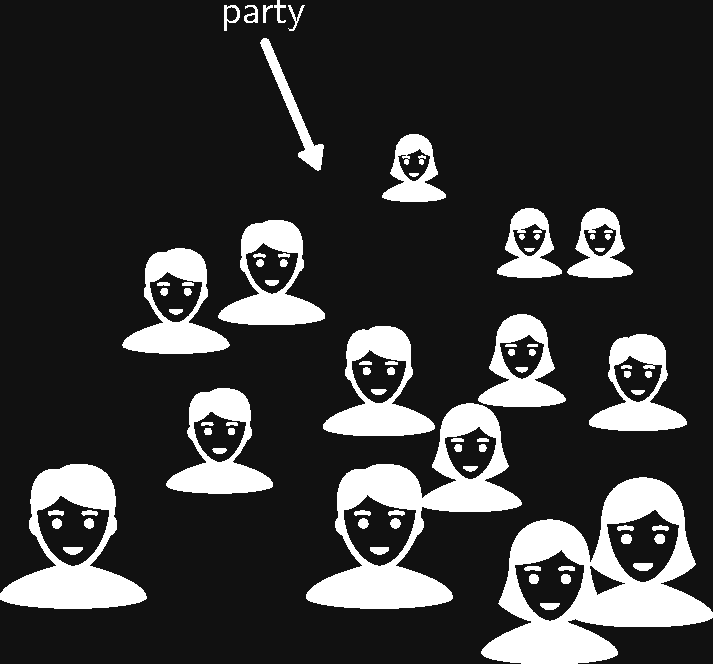
\includegraphics[width=5cm]{img/party.pdf}
	};
	\pdfcomment{Two analogies: One describing our expectations and one closer to the technical reality}
	\pdfcomment{We start by describing our expectations regarding conversation}
	\pdfcomment{Not everybody would automatically think of all points, but we want to establish them as a common ground}
\end{frame}

\begin{frame}
	\frametitle{A Private Room}
	You are now alone in a closed room with your Friend
	\begin{itemize}
		\item Both of you have absolute Confidentiality that you are alone
		\item Nobody can overhear your talk
		\item Your exchange is completely private
	\end{itemize}
	We call this \alert{confidentiality}

	\tikzoverlay at (current page.south east){
		
\includegraphics[width=6cm]{img/conversation.pdf}
	};

\end{frame}

\begin{frame}
	\frametitle{You Know Each Other}
	Since you're long-time friends, you're absolutely sure, whom you're talking to
	\begin{itemize}
		\item Nobody can impersonate your friend or you, without the other noticing
		\item You're talking directly, without a phone or webcam in between
	\end{itemize}
	We call this \alert{authenticity}
\end{frame}

\begin{frame}
	\frametitle{In Sight of Each Other}
	The room you're in is small enough that you can always see each other
	\begin{itemize}
		\item You know that the words you speak are received just as you spoke them
		\item There is no way either of you hears something other than the other says
	\end{itemize}
	We call this \alert{integrity}
\end{frame}

\begin{frame}
	\frametitle{It's a One-Time Talk}
	\only<1>{%
	Suppose somebody steps into the room
	\begin{itemize}
		\item They could overhear your conversation
		\item They would only learn the contents of this particular conversation
		\item They would not learn anything about past conversations you had
	\end{itemize}
	We call this \alert{forward secrecy}
	\begin{itemize}
		\item[$\rightarrow$] After leaving they would not be able to listen to any future conversations you might have
	\end{itemize}
	We call this \alert{future secrecy}}
	\pdfcomment{Future Secrecy is also called post-compromise security}
	\only<2>{%
		Forward- and Future Secrecy\\
		\begin{center}
			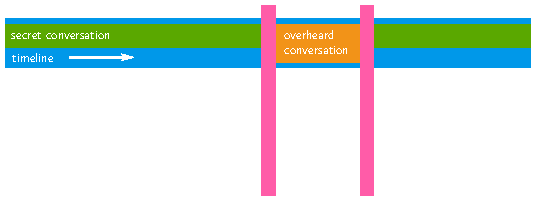
\includegraphics[width=\textwidth]{img/pfs-simple.pdf}
		\end{center}
	}
\end{frame}

\begin{frame}
	\frametitle{It's a One-Time Talk Between Only You Two}
	There are no witnesses in the room
	\begin{itemize}
		\item Either of you can later deny to other having made any statement
		\item Neither of you can prove to other that any of you have made a particular statement
	\end{itemize}
	We call this \alert{deniability}
\end{frame}

%\section{Enter Messaging Services}

\begin{frame}
	\frametitle{Messaging -- Reality Check}
	\only<1>{%
		\centering
		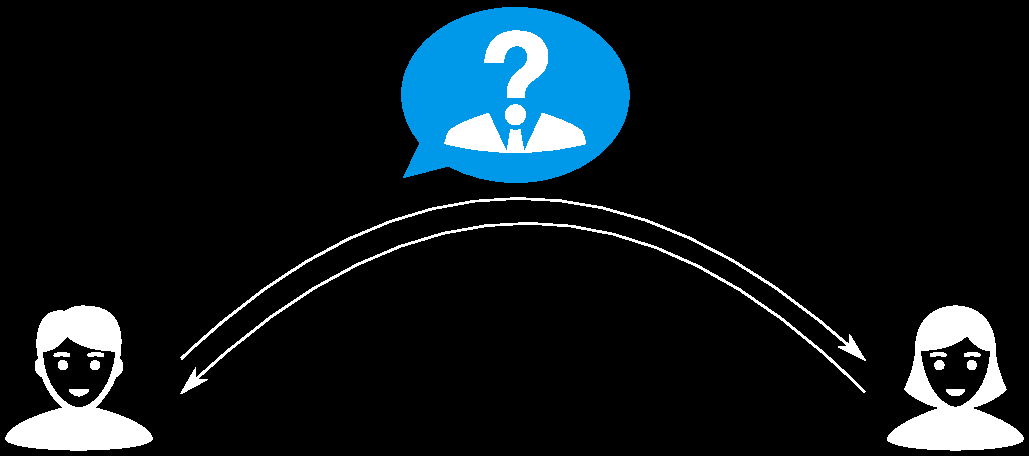
\includegraphics[width=.75\textwidth]{img/messaging.pdf}	
	}
	\pdfcomment{Now we have established our ideal scenario and want to check if this still applies to messaging.}
	\pdfcomment{This begins with the entry of a new player, the messaging service}
	\pdfcomment{This brings us to our second analogy, the one that describes messaging from a technical perspective}
	% \only<2>{%
	% 	Parties involved
	% 	\begin{itemize}
	% 		\item Depending on the scenario, at least one additional party is involved, the messaging provider
	% 		\item push message provider might also be involved
	% 		\item In federated scenarios, multiple relaying parties may be involved
	% 		\item[$\Rightarrow$] Messaging solutions should be designed so as to minimized the data these parties may obtain
	% 	\end{itemize}
	% 	Problems:
	% 	\begin{itemize}
	% 		\item How to find your peers? (address book leakage)
	% 		\item How to relay messages to the recipient? (participation leakage)
	% 		\item Relay always knows the exact time a message was sent
	% 		\item Relay always knows the size of transmitted messages (padding helps)
	% 	\end{itemize}
	% }
\end{frame}

\begin{frame}
	\frametitle{Messaging -- A More Technical Analogy}
		We started with a conversation analogy to identify our expectations of messaging\\[12pt]
		$\rightarrow$ Actually \alert{postal services} are better to look at messaging from a technical point of view.\\[24pt]
		\begin{center}
			\begin{tikzpicture}
				\node at (0,0) [anchor=east]   {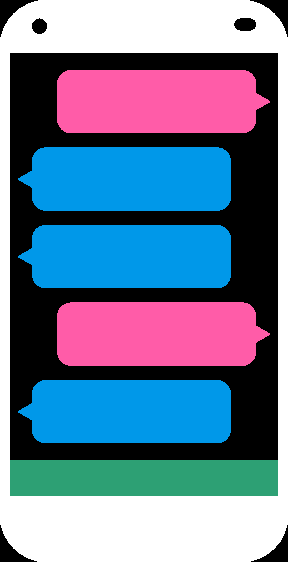
\includegraphics[width=2cm]{img/phone-chat.pdf}};
				\node at (2,0) [text height=2cm] {\fontsize{3cm}{3cm}\selectfont =\kern-.3ex>};
				\node at (4,0) [anchor=west]   {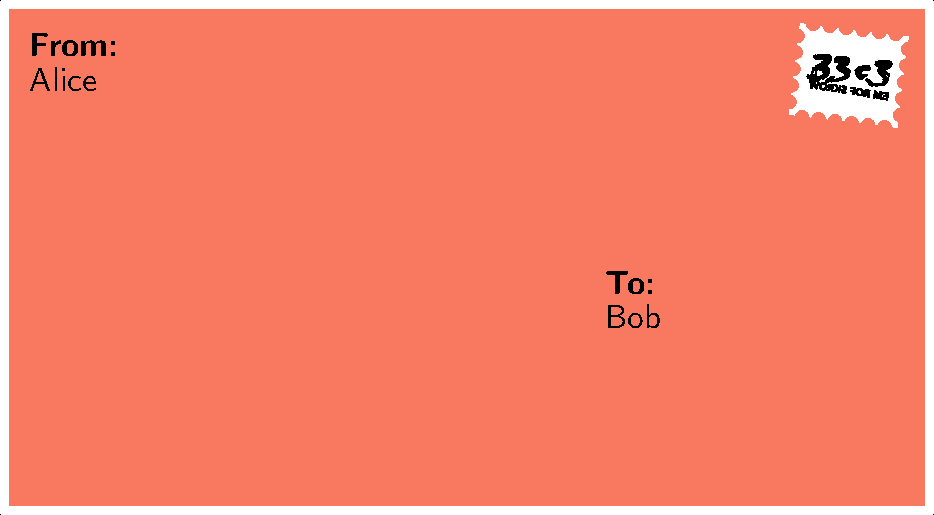
\includegraphics[width=5cm]{img/letter-example.pdf}};
			\end{tikzpicture}
		\end{center}
\end{frame}

\begin{frame}
	\frametitle{Example: Traditional Messaging}
	What if our party conversation had taken place via SMS?\\[1em]
	\begin{minipage}[t][.7\textheight]{\textwidth}
		\only<1>{\pdfcomment{As can be seen, our conversation analogy (and therefore our expectations) translates badly to the world of messaging. We need a new analogy. -- transition to next slide}
			Your providers (and other people on the same network)
			\begin{itemize}
				\item would know the contents of your exchange: \alert{no confidentiality}
				\item could change the contents of your exchange: \alert{no integrity}
				\item could reroute your messages and impersonate either of you: \alert{no authentication}
				%\item would know all messages you ever exchanged: \alert{no forward secrecy}
				%\item would know all messages exchanged in the future: \alert{no future secrecy}
				\item do not guarantee any secrecy, so we have neither \alert{forward secrecy} nor \alert{future secrecy}
				%\item could store all messages and use them as proof of the exchange: \alert{no deniability}
				\item[$\rightarrow$] We could argue having \alert{deniability} though.
			\end{itemize}
		}
	\end{minipage}
	\only<1->{$\rightarrow$ Messaging translates badly to our offline communication expectation}
	\pdfcomment{mobile messaging is like a postal service but feels like a private conversation}
\end{frame}

\begin{frame}
	\frametitle{From Postcards to Letters}
	\onslide<1->{
		\centering
		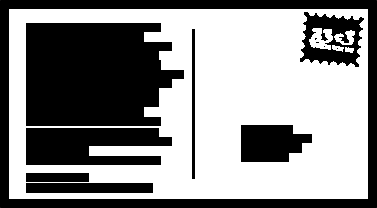
\includegraphics[width=.2\textwidth]{img/postcard.pdf}
		\-\\[2em]
	}
	\onslide<2>{
		\centering
		
\includegraphics[width=.3\textwidth]{img/letter-to-envelope.pdf}
		\pdfcomment{Now we have established an analogy of our expectations and one a bit closer to the communication reality. Now let's compare and evaluate both.}
		\pdfcomment{We start by looking at the envelope and asking how we can do that. -> Short encryption to cryptography.}
	}
\end{frame}

\begin{frame}[t]
	%weird constructs on this slide to prevent image jumping on overlay stepping
	\frametitle{The Shortest Introduction to Encryption You Will Ever Get}
		\vspace{-1ex}
		\onslide<1->{
			\begin{minipage}[t][.46\textheight]{\textwidth}
				Symmetric Encryption:\\
				\quad\small\alert{$\rightarrow$} Encryption and decryption  with the same key
				\begin{center}
					\only<1>{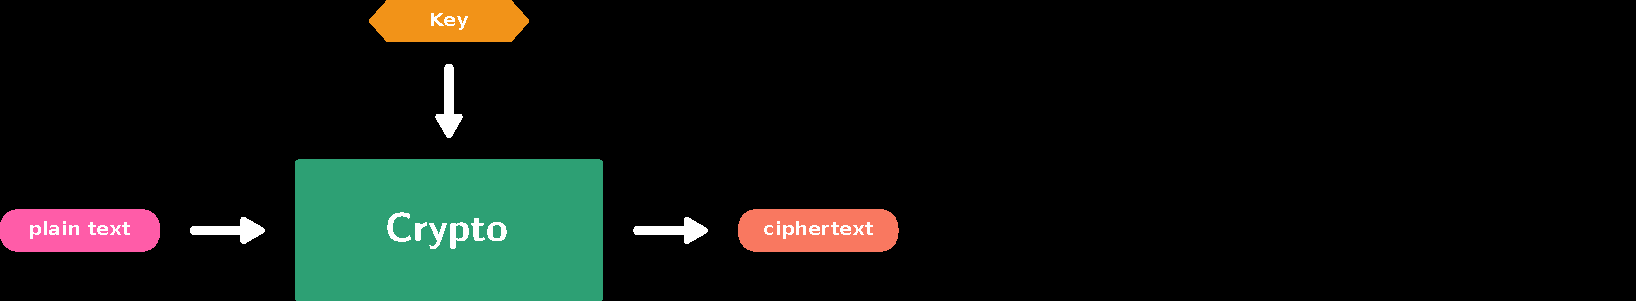
\includegraphics[width=.8\textwidth]{img/symmetric_crypto-1.pdf}\\[2ex]}
					\only<2->{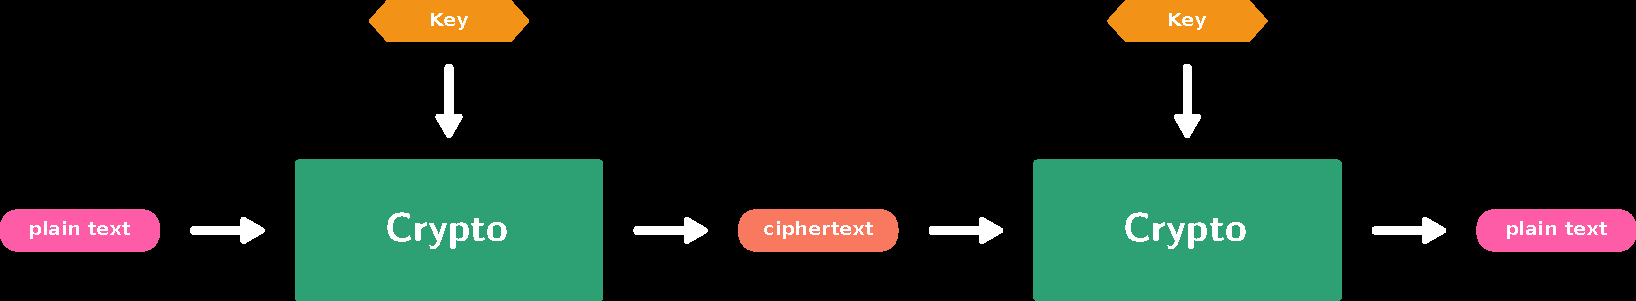
\includegraphics[width=.8\textwidth]{img/symmetric_crypto.pdf}\\[2ex]}
				\end{center}
		\end{minipage}
			}
		\onslide<3->{
			Asymmetric Encryption:\\
			\quad\small\alert{$\rightarrow$} Encryption and decryption with different keys
			\begin{center}
				\only<3>{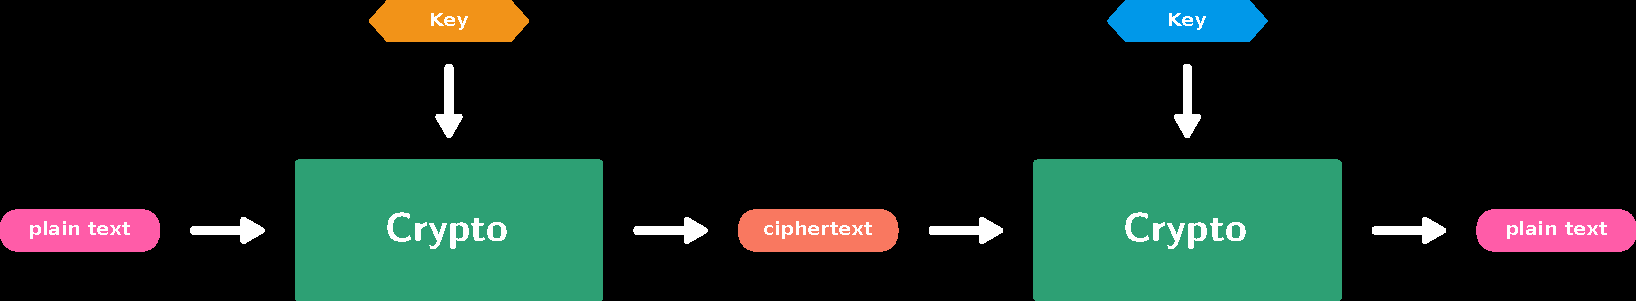
\includegraphics[width=.8\textwidth]{img/asymmetric_crypto.pdf}}
				\only<4>{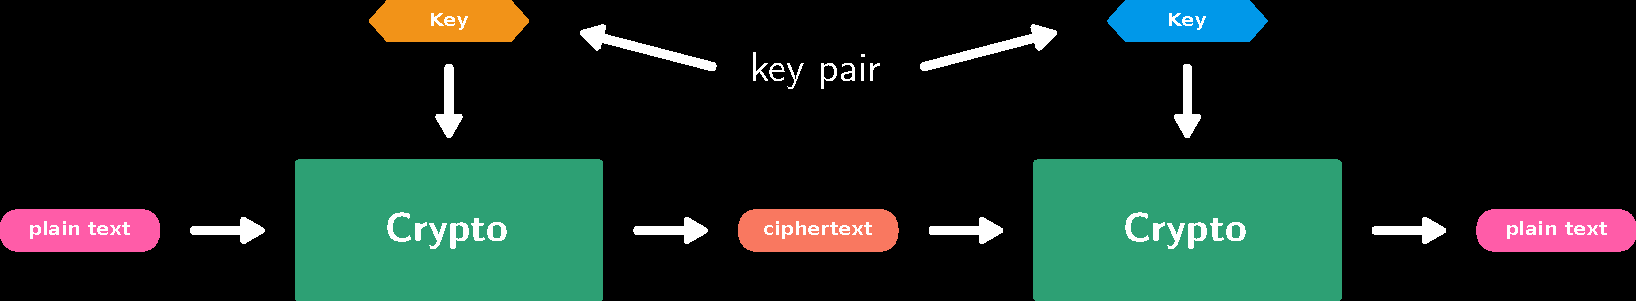
\includegraphics[width=.8\textwidth]{img/asymmetric_crypto-2.pdf}}
			\end{center}
		}
\end{frame}

\begin{frame}
	\frametitle{Public-Key Cryptography -- In a Nutshell}
	\vspace{3mm}
	\begin{minipage}[t][.65\textheight]{\textwidth}
		\begin{center}
			\only<1-2>{
				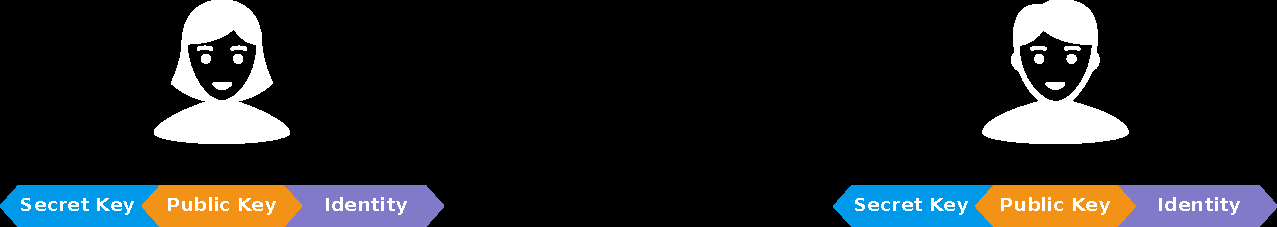
\includegraphics[width=\textwidth]{img/alice-bob-pki.pdf}\\[1.5em]
				\onslide<2>{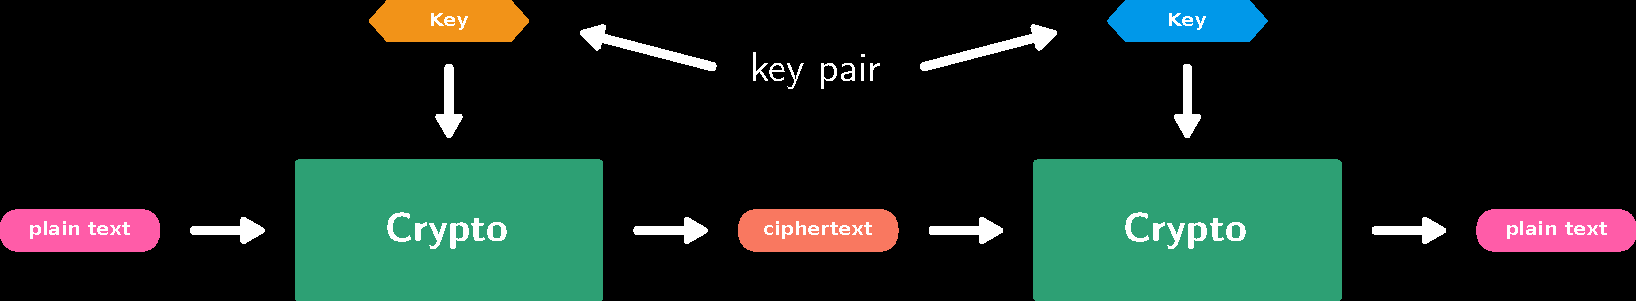
\includegraphics[width=.7\textwidth]{img/asymmetric_crypto-2.pdf}}
			}
			\only<3>{
				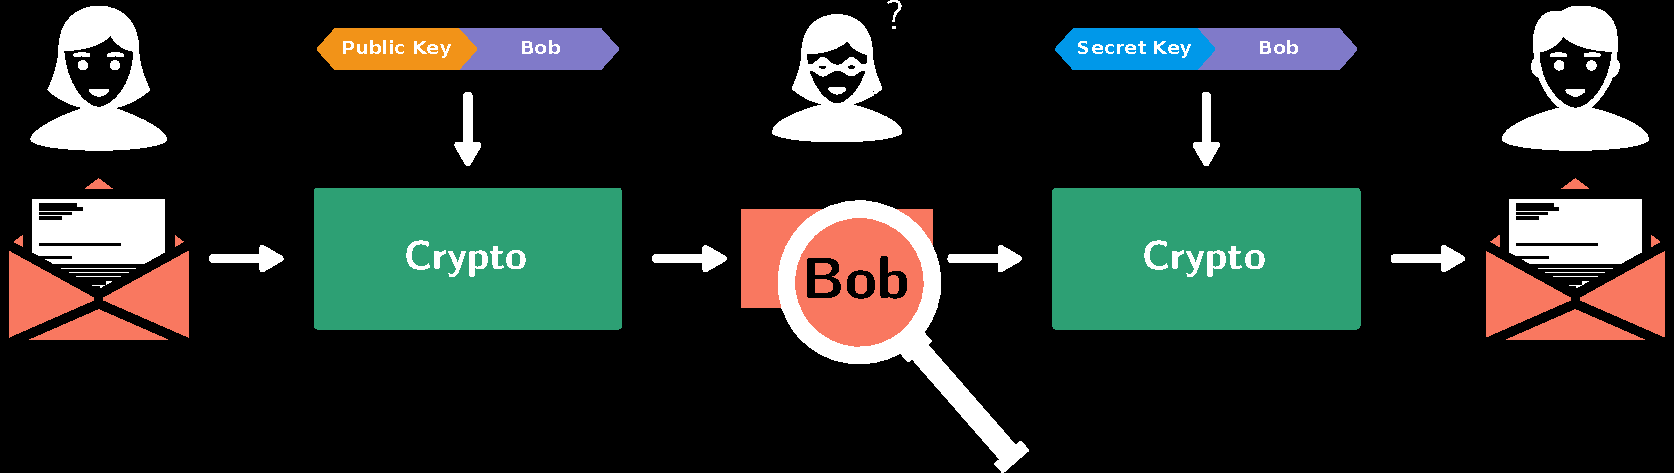
\includegraphics[width=\textwidth]{img/pki-msg-exchange.pdf}
			}
		\end{center}
	%\onslide<3->
	\end{minipage}

	\begin{itemize}
		\item Both parties publish their identities and public keys
		\item Any message can be encrypted with anyone's public key and only be decrypted with its corresponding secret key
	\end{itemize}
	\pdfcomment{This scheme is very expensive and a message can always be sent by anyone}
\end{frame}

\begin{frame}
	\frametitle{Key Establishment}
	\center
	\pdfcomment{what if we had a scheme, that produced a key specifically from one public and one private key}
	\pdfcomment{turns out, we have. And it works both ways and produces the same key}
	\pdfcomment{this is one particular way to perform key agreement}
	\pdfcomment{as we will later see, there is a better way consisting of a 4-way message exchange. But for that, both parties have to be online}.
	\pdfcomment{this scheme has one advantage and one disadvantage. The advantage was just mentioned, the disadvantage is that we always come up with the same key. And we will see why that is a problem in a minute}
	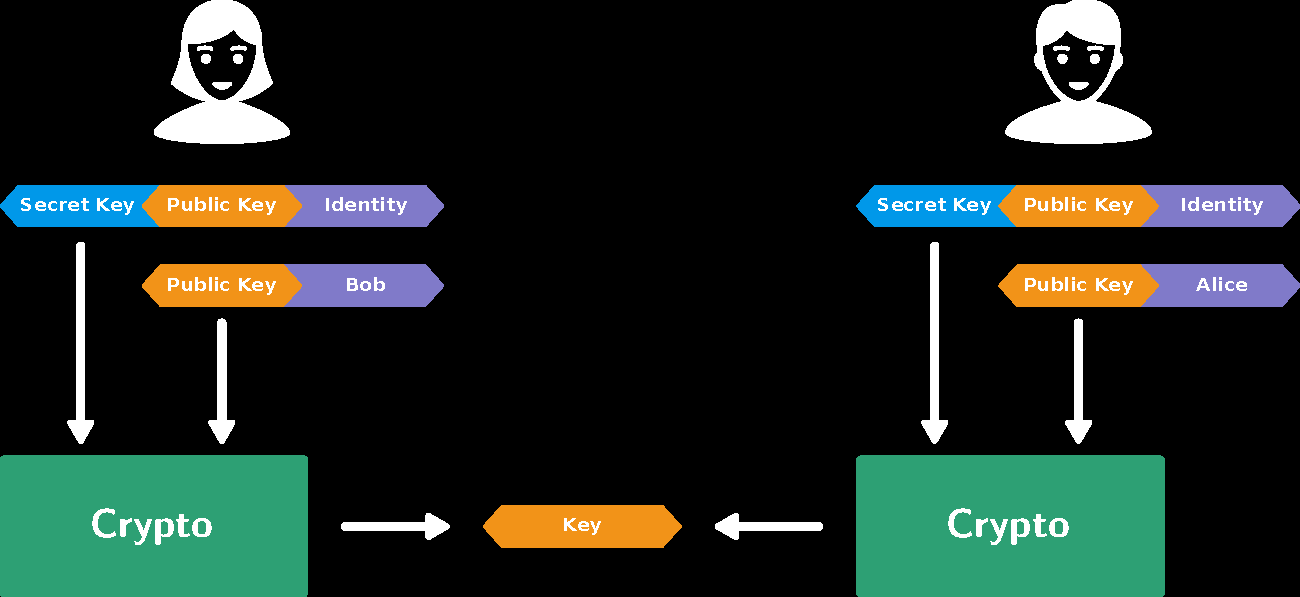
\includegraphics[width=.9\textwidth]{img/pka.pdf}	
\end{frame}

\begin{frame}
	\frametitle{Recap}
	%\begin{itemize}
	%	\item \alert{Asymmetric Encryption} gives us IDs but is very expensive.\\[6pt]
	%		\begin{center}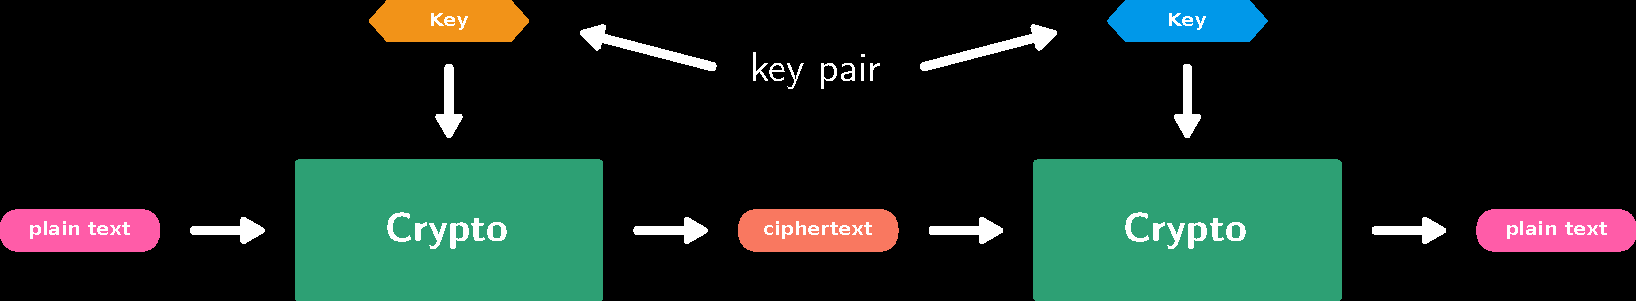
\includegraphics[width=.4\textwidth]{img/asymmetric_crypto-2.pdf}\end{center}

	%	\item \alert{Symmetric Encryption} is cheap, but a key has to be shared by all participants \alert{before} communication starts.
	%		\begin{center}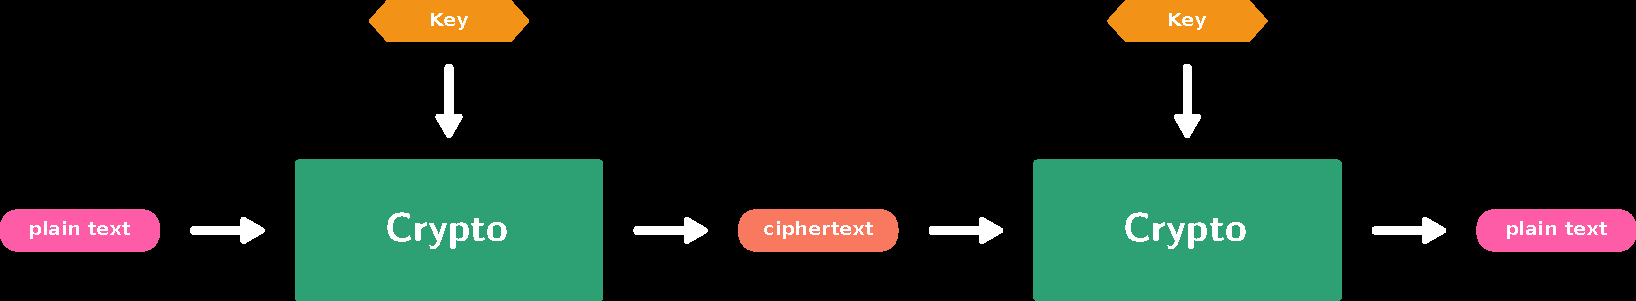
\includegraphics[width=.4\textwidth]{img/symmetric_crypto.pdf}\end{center}\\[12pt]
	%	\item \alert{Authenticated Encryption} allows us to create symmetric keys based on asymmetric key pairs.
	%\end{itemize}
	\begin{tabular}{@{}p{.6\textwidth}p{.4\textwidth}}
		\parbox{.6\textwidth}{\alert{Asymmetric Encryption} gives us IDs but is very expensive.} & \parbox{.4\textwidth}{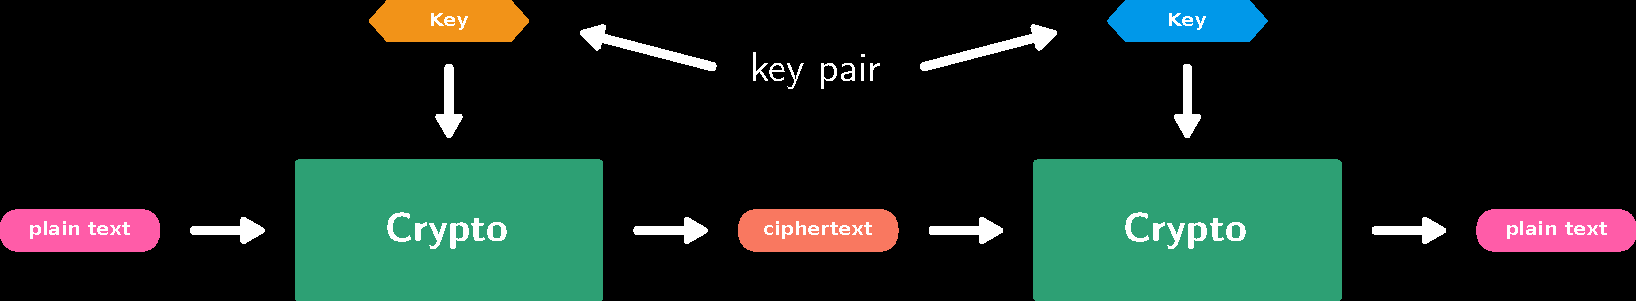
\includegraphics[width=.4\textwidth]{img/asymmetric_crypto-2.pdf}}  \\[36pt]
		\parbox{.6\textwidth}{\alert{Symmetric Encryption} is cheap, but a key has to be shared by all participants \alert{before} communication starts.} & \parbox{.4\textwidth}{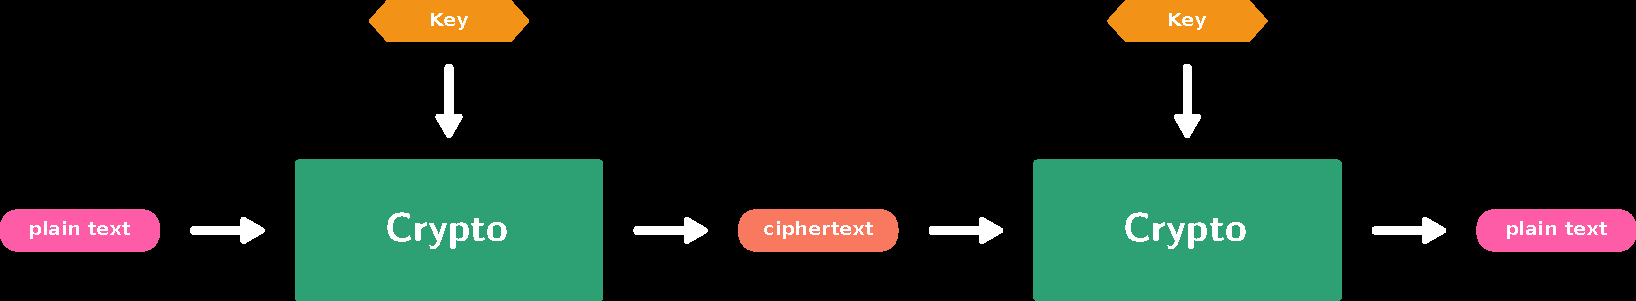
\includegraphics[width=.4\textwidth]{img/symmetric_crypto.pdf}} \\[36pt]
		\parbox{.6\textwidth}{\alert{Key Agreement} allows us to create symmetric keys based on asymmetric key pairs.} & \parbox{.4\textwidth}{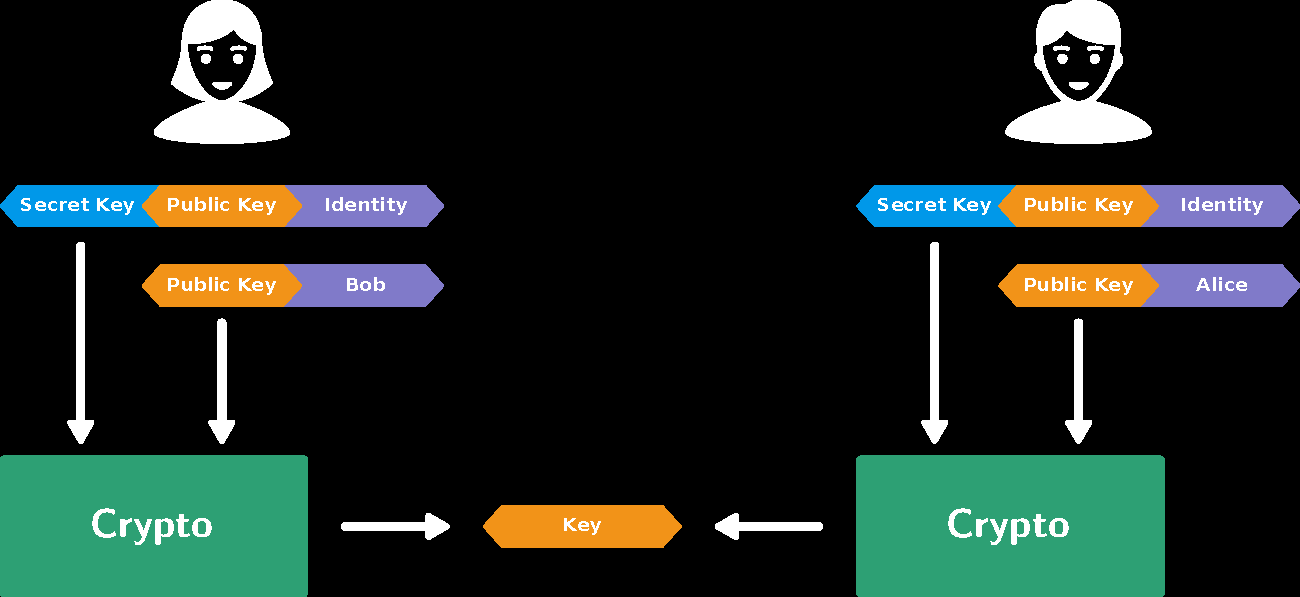
\includegraphics[width=.4\textwidth]{img/pka.pdf}} \\
	\end{tabular}
	\vfill
	But there's more\ldots
\end{frame}

\begin{frame}
	\frametitle{Confidentiality}
	\centering
	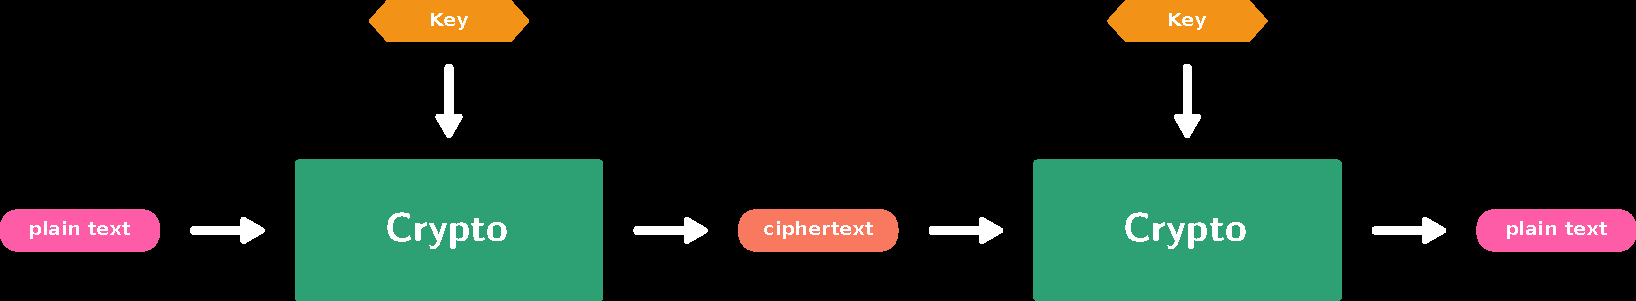
\includegraphics[width=.8\textwidth]{img/symmetric_crypto.pdf}\\[2em]
	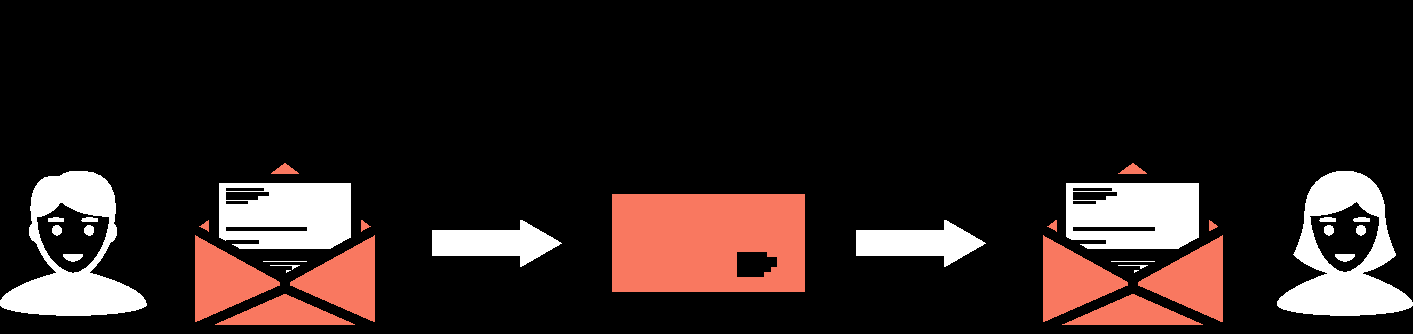
\includegraphics[width=.8\textwidth]{img/confidentiality.pdf}
	\pdfcomment{we can take our symmetric key (the one obtained from our authenticated encryption scheme) to obtain confidentiality}
\end{frame}

\begin{frame}
	\frametitle{Deniability}
	\only<1>{
		\centering
		\-\\[.5em]
		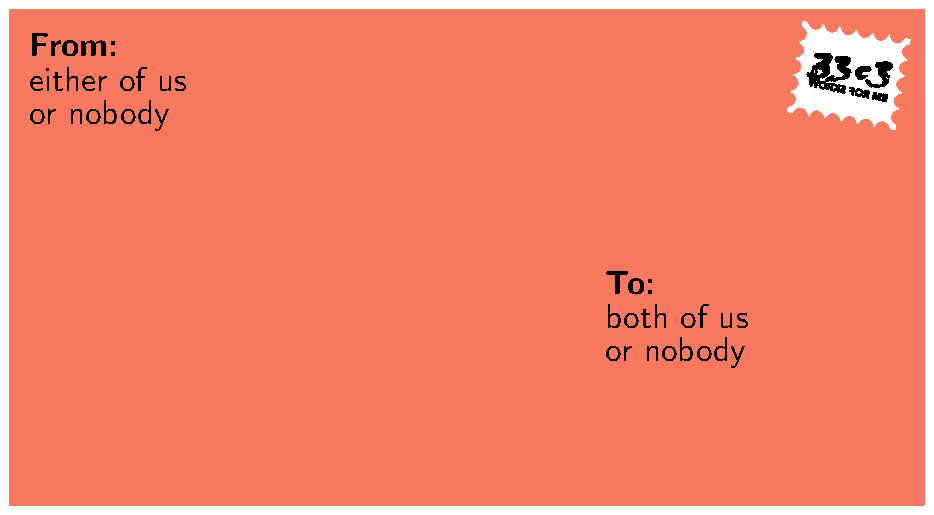
\includegraphics[width=.8\textwidth]{img/deniability-letter.pdf}
		\pdfcomment{Public-Key Authenticators einfach erklären für Deniability}
	}
	%\begin{overlayarea}{\textwidth}{\textheight}
	%	\begin{itemize}
	%		\item<2-> In asymmetric cryptography, it is always clear who sent a message, once the protocol is broken on either side
	%		\item<3-> It can, however, be used to exchange a symmetric key that either parties share
	%		\item<4-> Now either Party can deny authoring any message
	%	\end{itemize}
	%	\-\\
	%	\begin{center}
	%		\only<2>{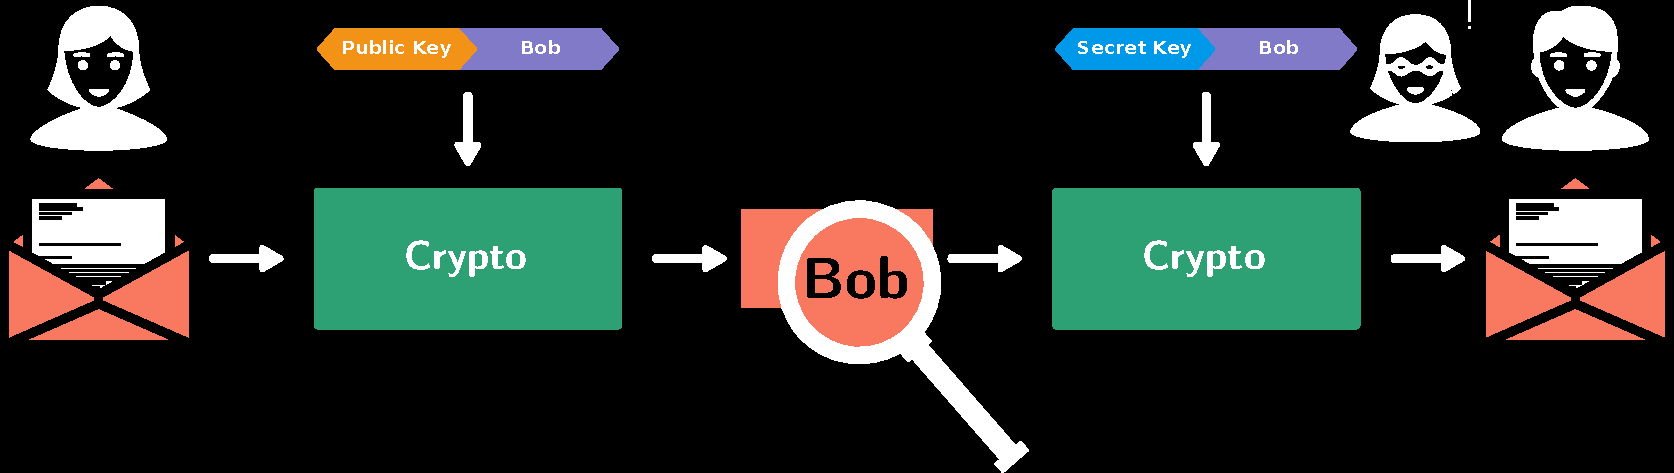
\includegraphics[width=.8\textwidth]{img/no-deniability.pdf}\pdfcomment{now our hacker has managed to break into Bob's phone and can look at the messages}}
	%		\only<3->{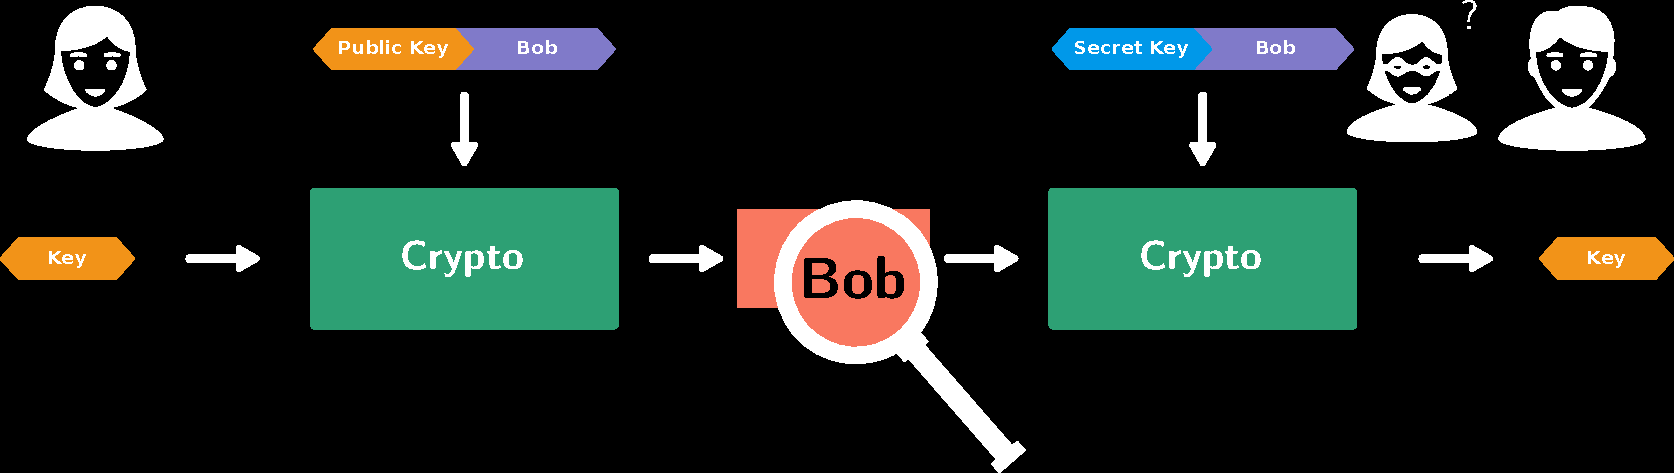
\includegraphics[width=.8\textwidth]{img/key-agreement.pdf}}
	%	\end{center} 
	%\end{overlayarea} 
\end{frame} 

\begin{frame}
	\frametitle{But What About Forward- and Future Secrecy?}
	\begin{center}
		\only<1>{\pdfcomment{We remember our simple explanation of PFS}
			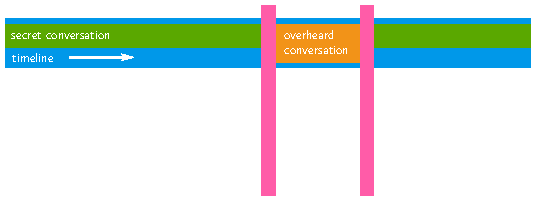
\includegraphics[width=\textwidth]{img/pfs-simple.pdf}
		}
		\only<2>{\pdfcomment{now we transfer this image to messaging}
			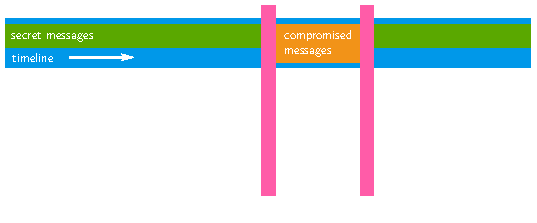
\includegraphics[width=\textwidth]{img/pfs.pdf}
		}
		\pdfcomment{The easiest way to do this is to discard each key after one use and exchange a new one}
		\pdfcomment{Of course this has to happen in a way that no attacker with a stolen key learns anything about the next one}
		\onslide<3->{
			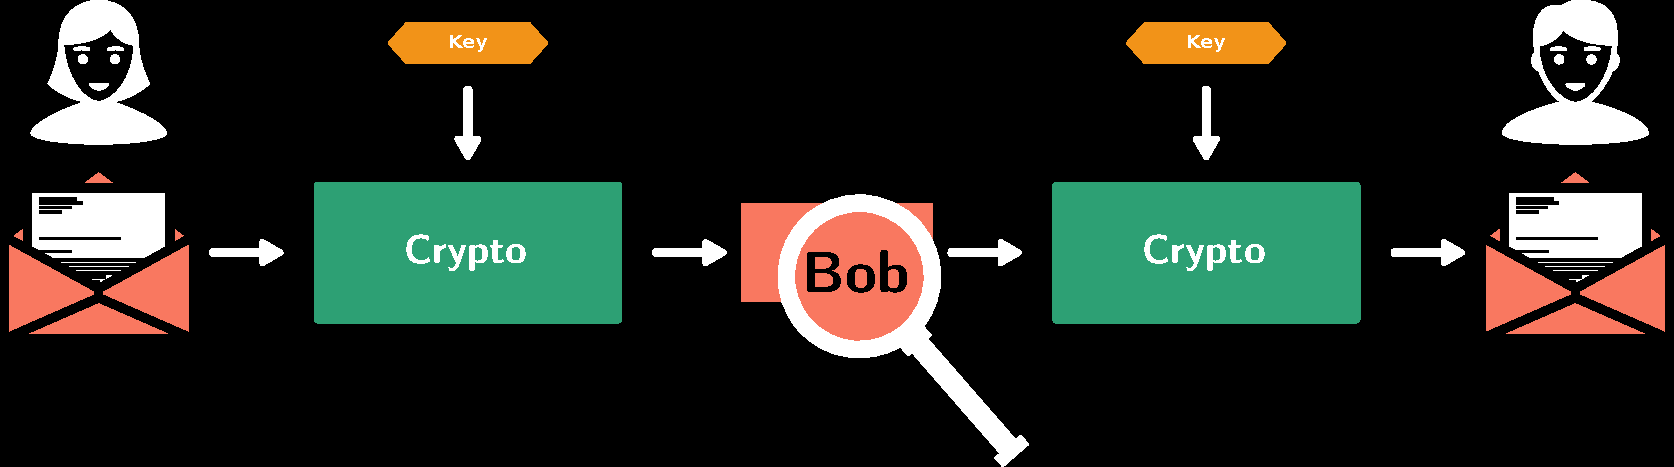
\includegraphics[width=.9\textwidth]{img/e2e-symmetric.pdf}
			\-\\[1em]\pause
		}
		\onslide<4->{
			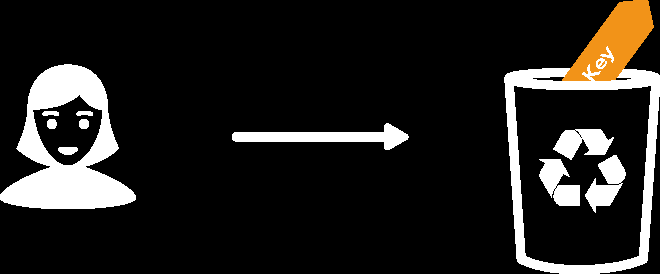
\includegraphics[width=.4\textwidth]{img/discard-key.pdf}
		}
	\end{center}
	\pdfcomment{Since we get our key from both secret and public keys, we cannot simply discard it.}
	\pdfcomment{Therefore we don't have PFS in the scheme we have sketched now.}
	\pdfcomment{We could get it back, though, if we had a way to renegotiate public- and secret keys.}
\end{frame}

\begin{frame}
	\frametitle{Recap}
	Our key agreement protocol gives us:
	\begin{itemize}
		\item Confidentiality
		\item Deniability
		\item Authenticity
	\end{itemize}
	We don't have:
	\begin{itemize}
		\item Forward Secrecy
		\item Future Secrecy
	\end{itemize}
	\-\\[2em]
	\alert{$\rightarrow$} We are ignoring Integrity here, but we have that, too.
\end{frame}

\begin{frame}
	\frametitle{Key and ID Management}
	\only<1>{%
		\centering
		\begin{block}{}
			Cryptography is rarely, if ever, the solution to a security problem. Cryptography is a translation mechanism, usually converting a communications security problem into a key management problem.\\
			\hfill ---Dieter Gollmann
		\end{block}
	}
	\only<2>{%
		\centering
		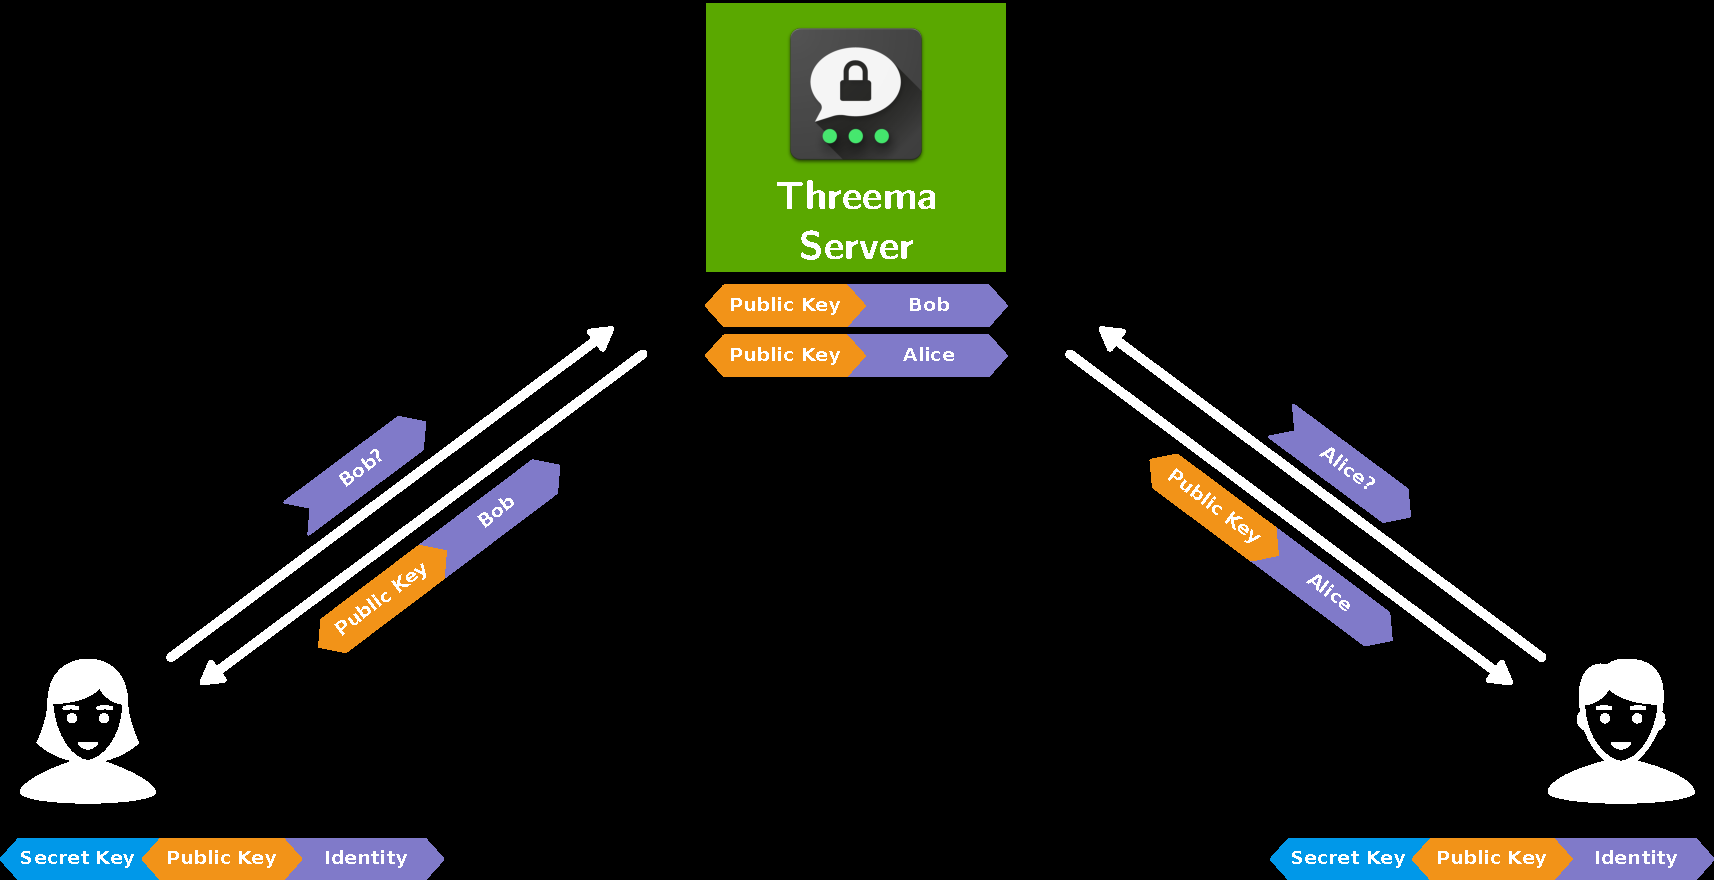
\includegraphics[width=.9\textwidth]{img/identity-query.pdf}
		\pdfcomment{Messengers try to solve this problem by introducing a central repository of IDs and public keys}
		\pdfcomment{User can query this server and ask for public keys and IDs}
		\pdfcomment{But this only solves part of our problem}
	}
	\only<3-7>{%
		We can ask for IDs, but what is an ID?
		\begin{itemize}
			\item A phone number?\\
				\onslide<4->{\quad\alert{$\rightarrow$} Can identify a user. But is also considered personal information.}
			\item An email address?\\
				\onslide<5->{\quad\alert{$\rightarrow$} Same thing as with phone number. But a temporary email can be used.}
			\item Something else?\\
				\onslide<6->{\quad\alert{$\rightarrow$} Dedicated IDs offer anonymous usage, but ID ownership must be verifyable.}
		\end{itemize}
		\vfill
		\onslide<7->{$\rightarrow$ \alert{Dedicated IDs are preferrable. But only if we find a way to verify ID ownership}}
	}
	\only<8>{%
		How does Alice know which is Bob's public key?\\[3em]
		\begin{center}
			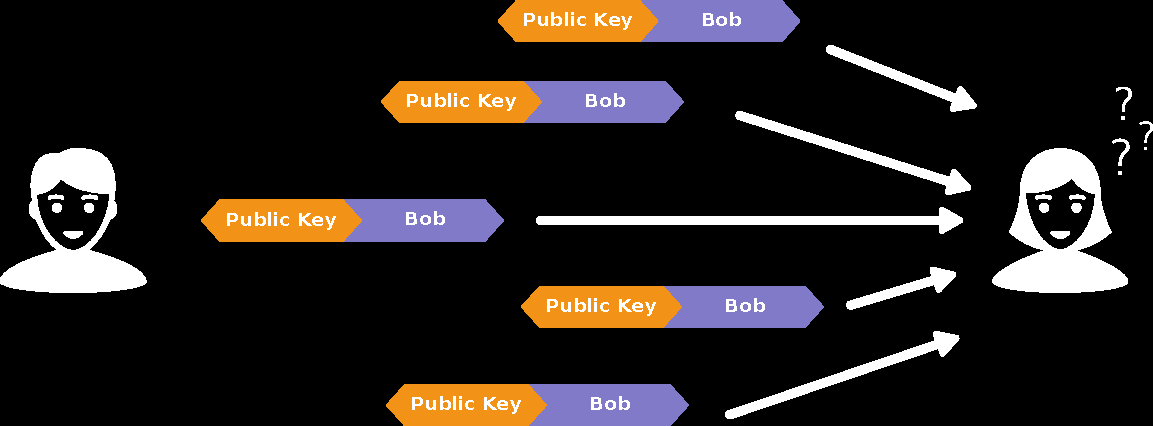
\includegraphics[width=.5\textwidth]{img/alice-confused-by-bobs-ids.pdf}
		\end{center}
		\pdfcomment{We have now connected Bob's ID using his phone number that we know}
		\pdfcomment{But we still put all our trust in the messenger directory}
		\pdfcomment{At this point we depend on Bob's provider for the right phone number and the messenger for its connection to Bob's ID}
			%\item Identity keys stored on devices, what if stolen
			%\item Keys for back-end communication layer hard-coded, almost impossible to replace
			%\item How to deal with key compromise? (answer: key rotation)
	}
\end{frame}

\begin{frame}
	\frametitle{Mobile Messaging Key Management}
	\-\\
	\begin{overlayarea}{\textwidth}{\textheight}
		\only<1>{
			\centering
			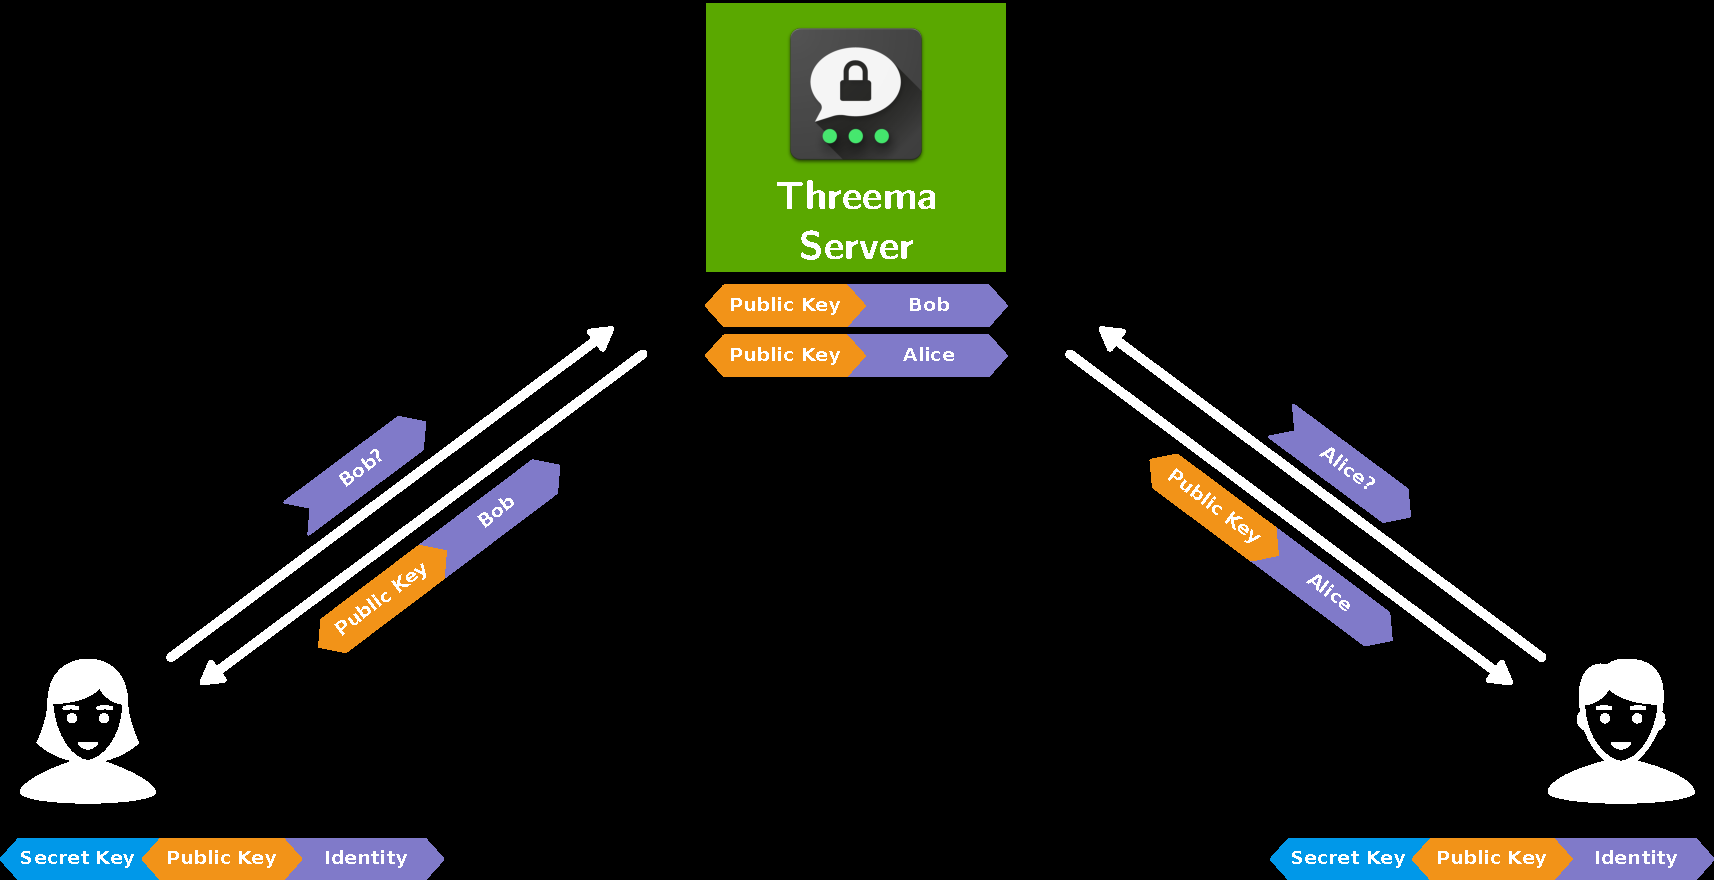
\includegraphics[width=.9\textwidth]{img/identity-query.pdf}
		}
		\only<2>{
			\centering
			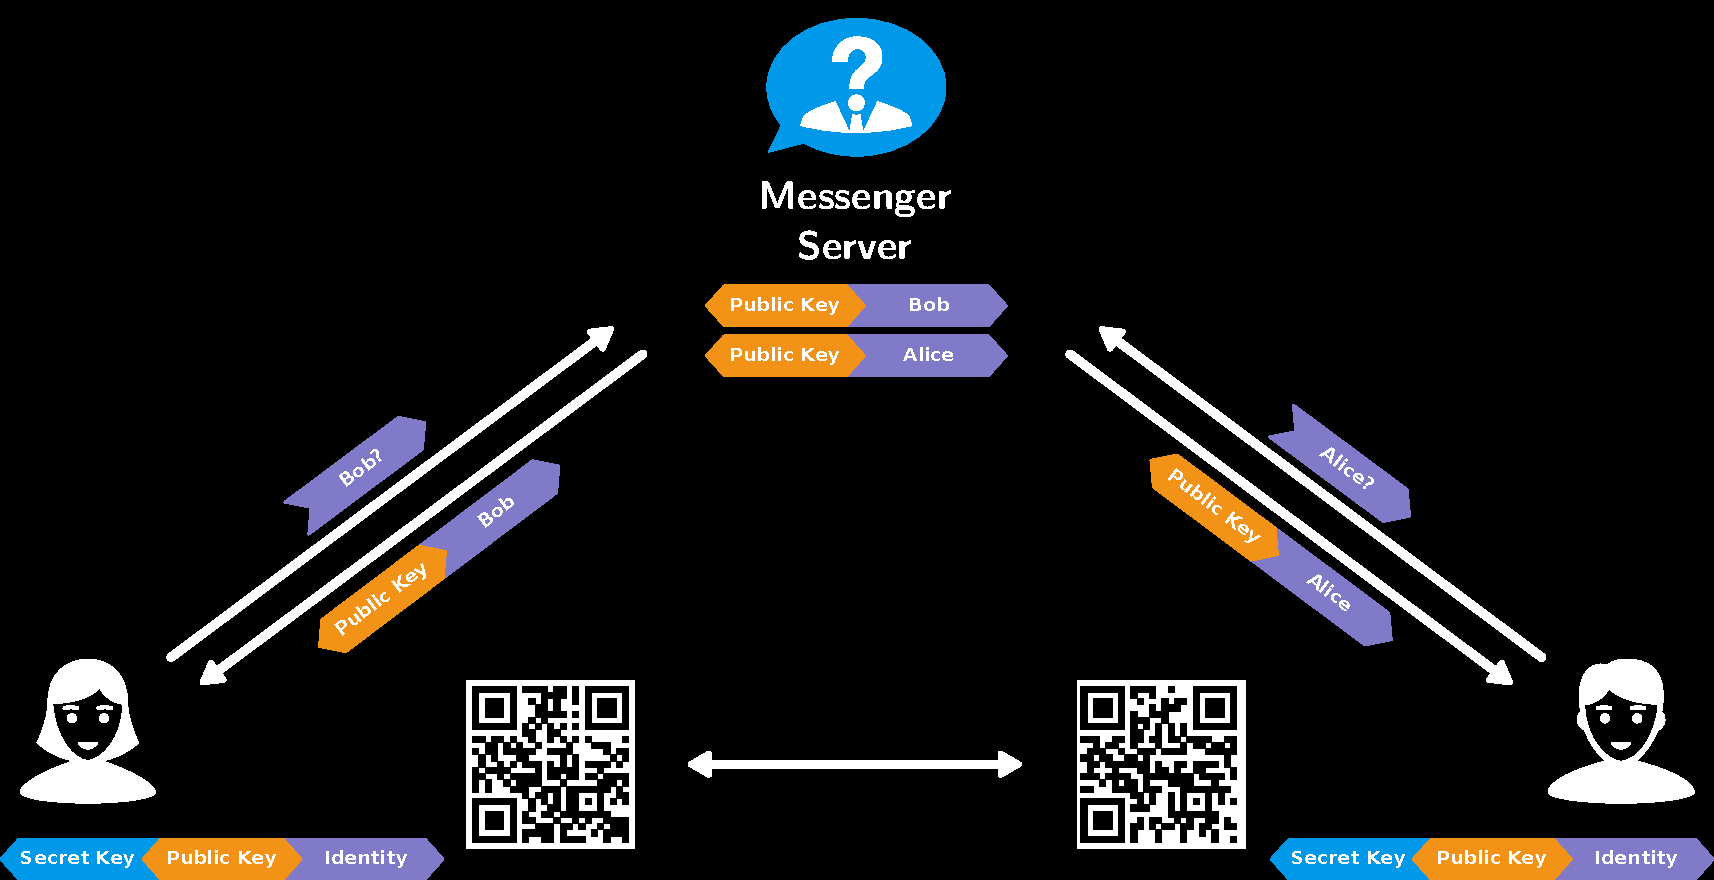
\includegraphics[width=.9\textwidth]{img/identity-query2.pdf}
		}
	\end{overlayarea}
	
\end{frame}

\begin{frame}
	\frametitle{Authenticity}
	We have now solved the Authentiticy problem
	\begin{itemize}
		\item User can be identified by their phone number or email address\\
			\quad\alert{$\rightarrow$} But they have dedicated IDs.\\
			\quad\alert{$\rightarrow$} Personal verification is possible.
	\end{itemize}
	\vspace{2em}
	The remaining unsolved problem is a user changing their ID.\\
			\quad\alert{$\rightarrow$} At this point, the problem starts anew.\\
			\quad\alert{$\rightarrow$} We will get back to that later.
	%\begin{itemize}
	%	\item How to connect a key to a person?
	%		\begin{itemize}
	%			\item[$\rightarrow$] Key signing (PGP)
	%			\item[$\rightarrow$] Certificates (trusted third party)
	%			\item[$\rightarrow$] (Messenger-)service-based directory (based on phone numbers or email addresses)
	%				\pdfcomment{It is not a good idea to use phone numbers for identities, we rather want a separate ID. That's where Threema's approach is interesting}
	%		\end{itemize}
	%	\item How to deal with changing keys?
	%		\begin{itemize}
	%			\item warnings are annoying
	%			\item Threema's traffic light system encourages authentication but doesn't deal with changing keys (other than new identities for known phone numbers with yellow dots)
	%		\end{itemize}

	%\end{itemize}
\end{frame}

\begin{frame}
	\frametitle{Metadata Handling}
	\only<1>{%
		Everybody on the network can see:
		\begin{itemize}
			\item\alert{the sender} of the message
			\item\alert{the intended receiver} of the message
				\pdfcomment{They can also log the time and the size of the messages}
		\end{itemize}
		\begin{center}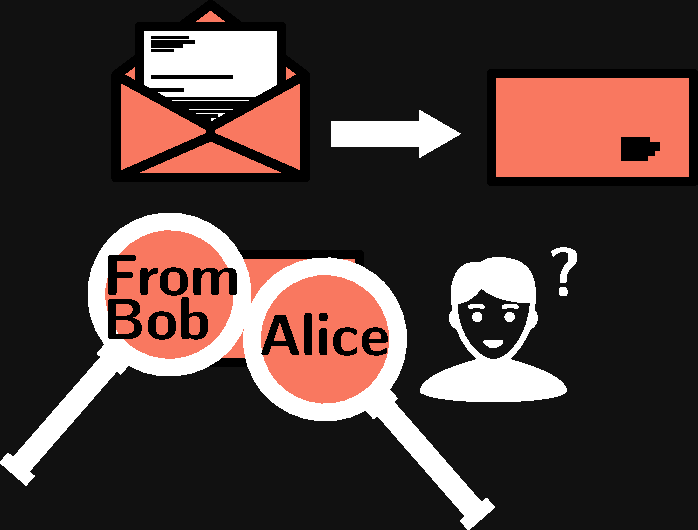
\includegraphics[width=5cm]{img/metadata-leak.pdf}\end{center}
	}
	\only<2>{
		Solution: wrap encrypted message in a second layer of encryption and address it only to the message server.
		\begin{center}
			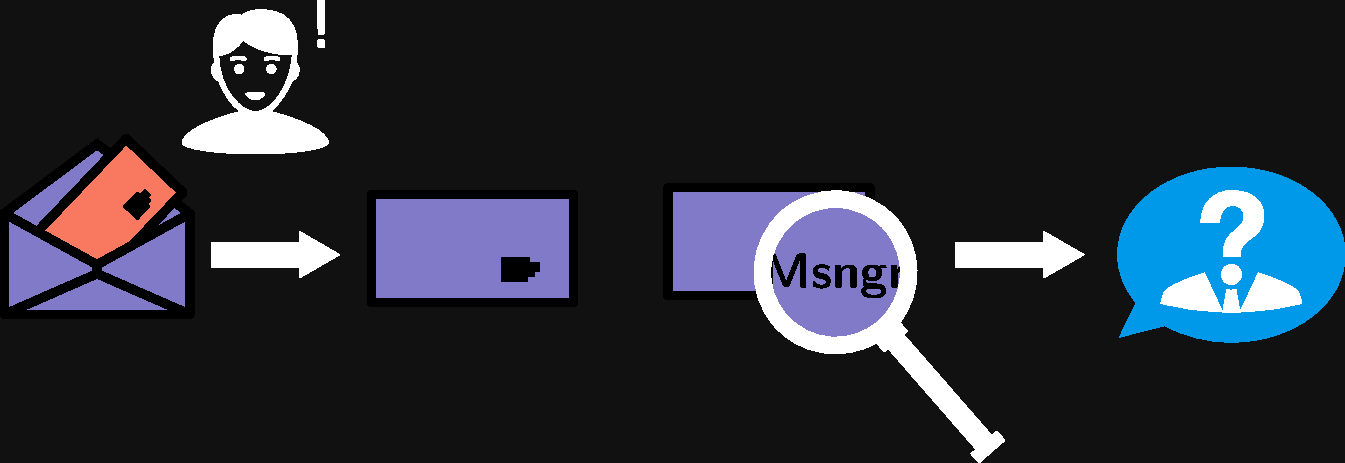
\includegraphics[width=.8\textwidth]{img/transport-layer-encryption.pdf}
		\end{center}
	}
	\only<3>{
		\begin{center}
			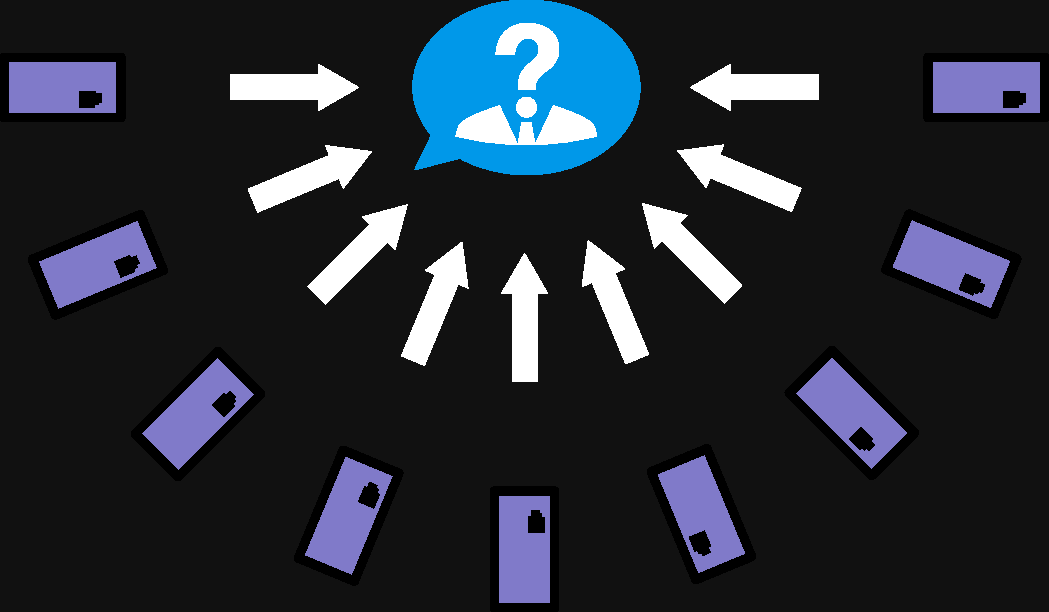
\includegraphics[width=.8\textwidth]{img/everybody-sends.pdf}
		\end{center}
	}
	\only<4>{
		\begin{center}
			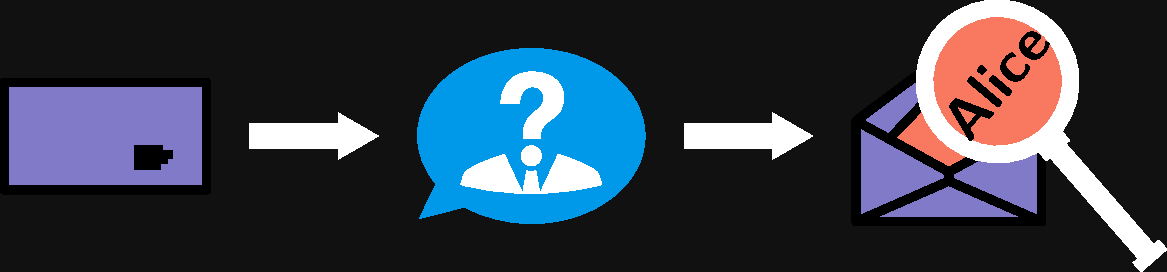
\includegraphics[width=.8\textwidth]{img/transport-layer-encryption-forwarding.pdf}
		\end{center}
	}
	\only<5>{
		The message server will remove the outer layer and add a new one, targeted at the receiver.
		\begin{center}
			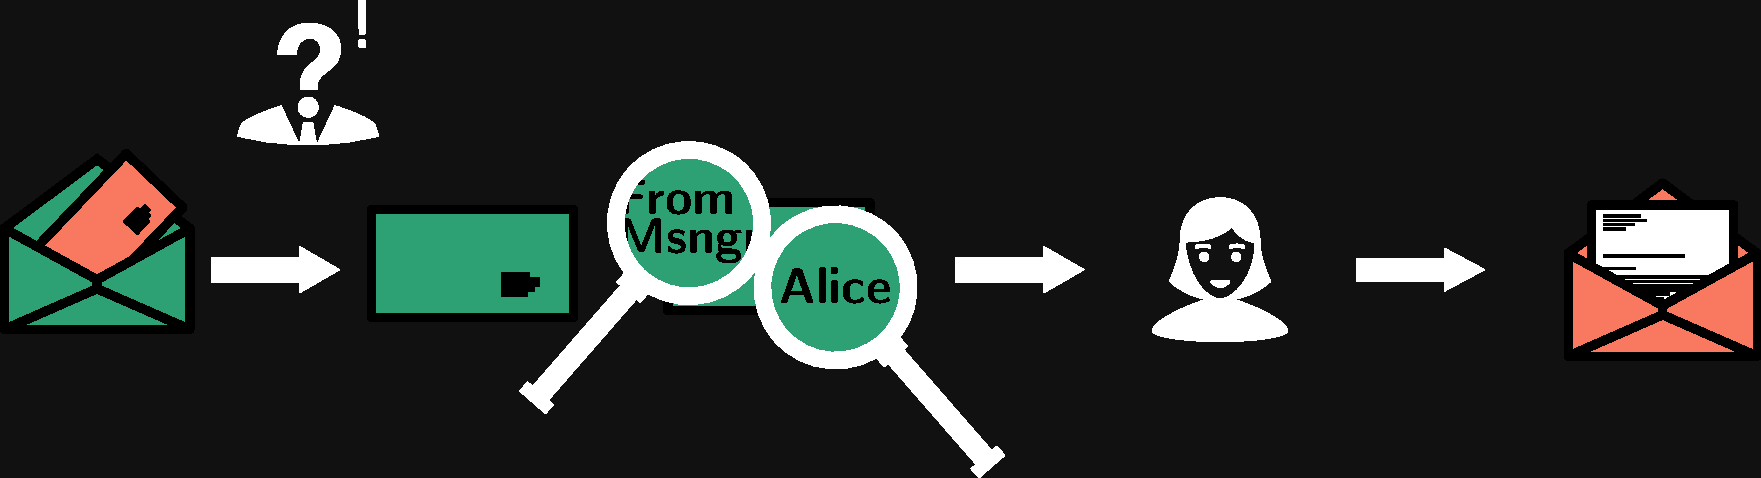
\includegraphics[width=.8\textwidth]{img/transport-layer-encryption-receiving.pdf}
		\end{center}
	}
	\only<6>{
		This leaves us with an encrypted \alert{end-to-end tunnel}, transmitted through two \alert{transport layer} encryption tunnels.\\
		\vspace{1cm}
		\begin{center}
			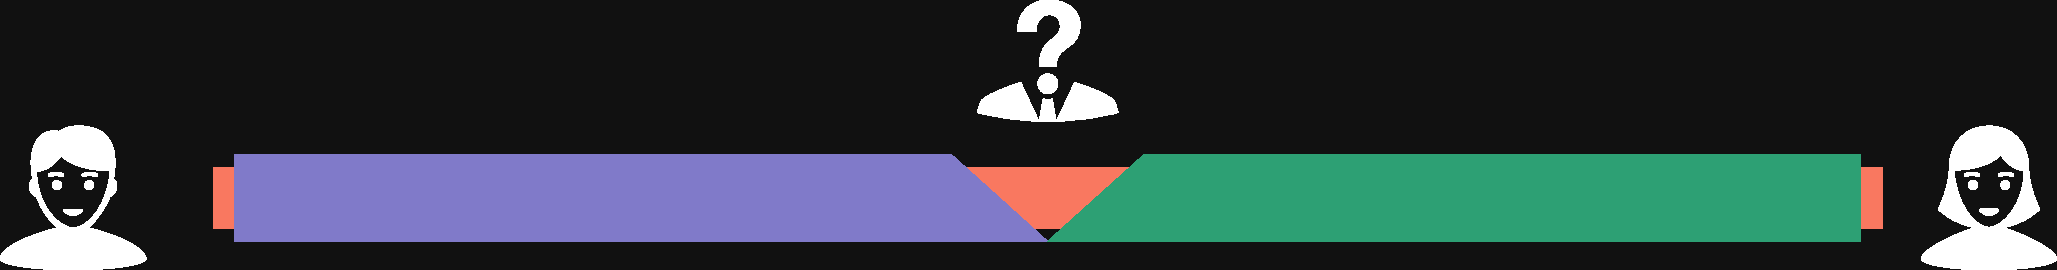
\includegraphics[width=\textwidth]{img/2-layer-tunnel.pdf}
		\end{center}
		\vspace{1cm}
		\alert{The message server still knows both communication partners!}
	}
		\only<7->{
			We can obfuscate the size of a message with \alert{padding}\\
			\-\\[2em]
		}
	\begin{overlayarea}{\textwidth}{\textheight}
		\only<8>{
			\begin{center}
				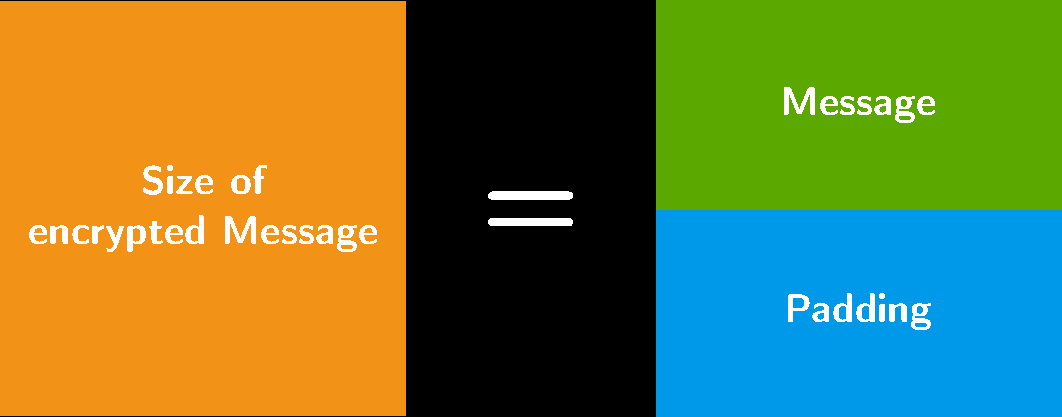
\includegraphics[width=.7\textwidth]{img/padding.pdf}
			\end{center}
			\pdfcomment{Of course padding should be randomly different every time}
		}

		% \onslide<9>{
		% 	\begin{center}
		% 		\includegraphics[page=13,clip,trim={.99cm 7.5cm 5cm 1cm},width=.9\textwidth]{out/messages.pdf}
		% 	\end{center}
		% }
	\end{overlayarea}
\end{frame}

\begin{frame}
	\frametitle{Threema}
	\centering
	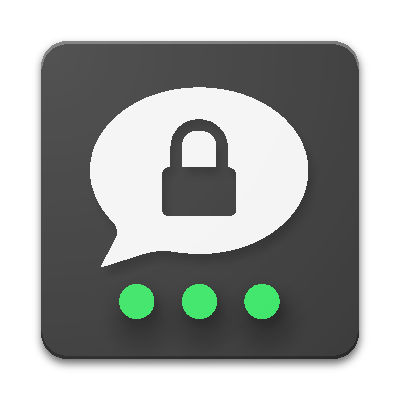
\includegraphics[width=.4\textwidth]{img/threema-android-icon-noshadow.pdf}
	\pdfcomment{no advertising}
	\pdfcomment{no recommendations}
	\pdfcomment{no formal analysis}
	\pdfcomment{it is closed-source so we could only work with that}
	\pdfcomment{we have looked at the app and will now present our findings}
\end{frame}

\begin{frame}
	\frametitle{Threema's Architecture}
	\centering
	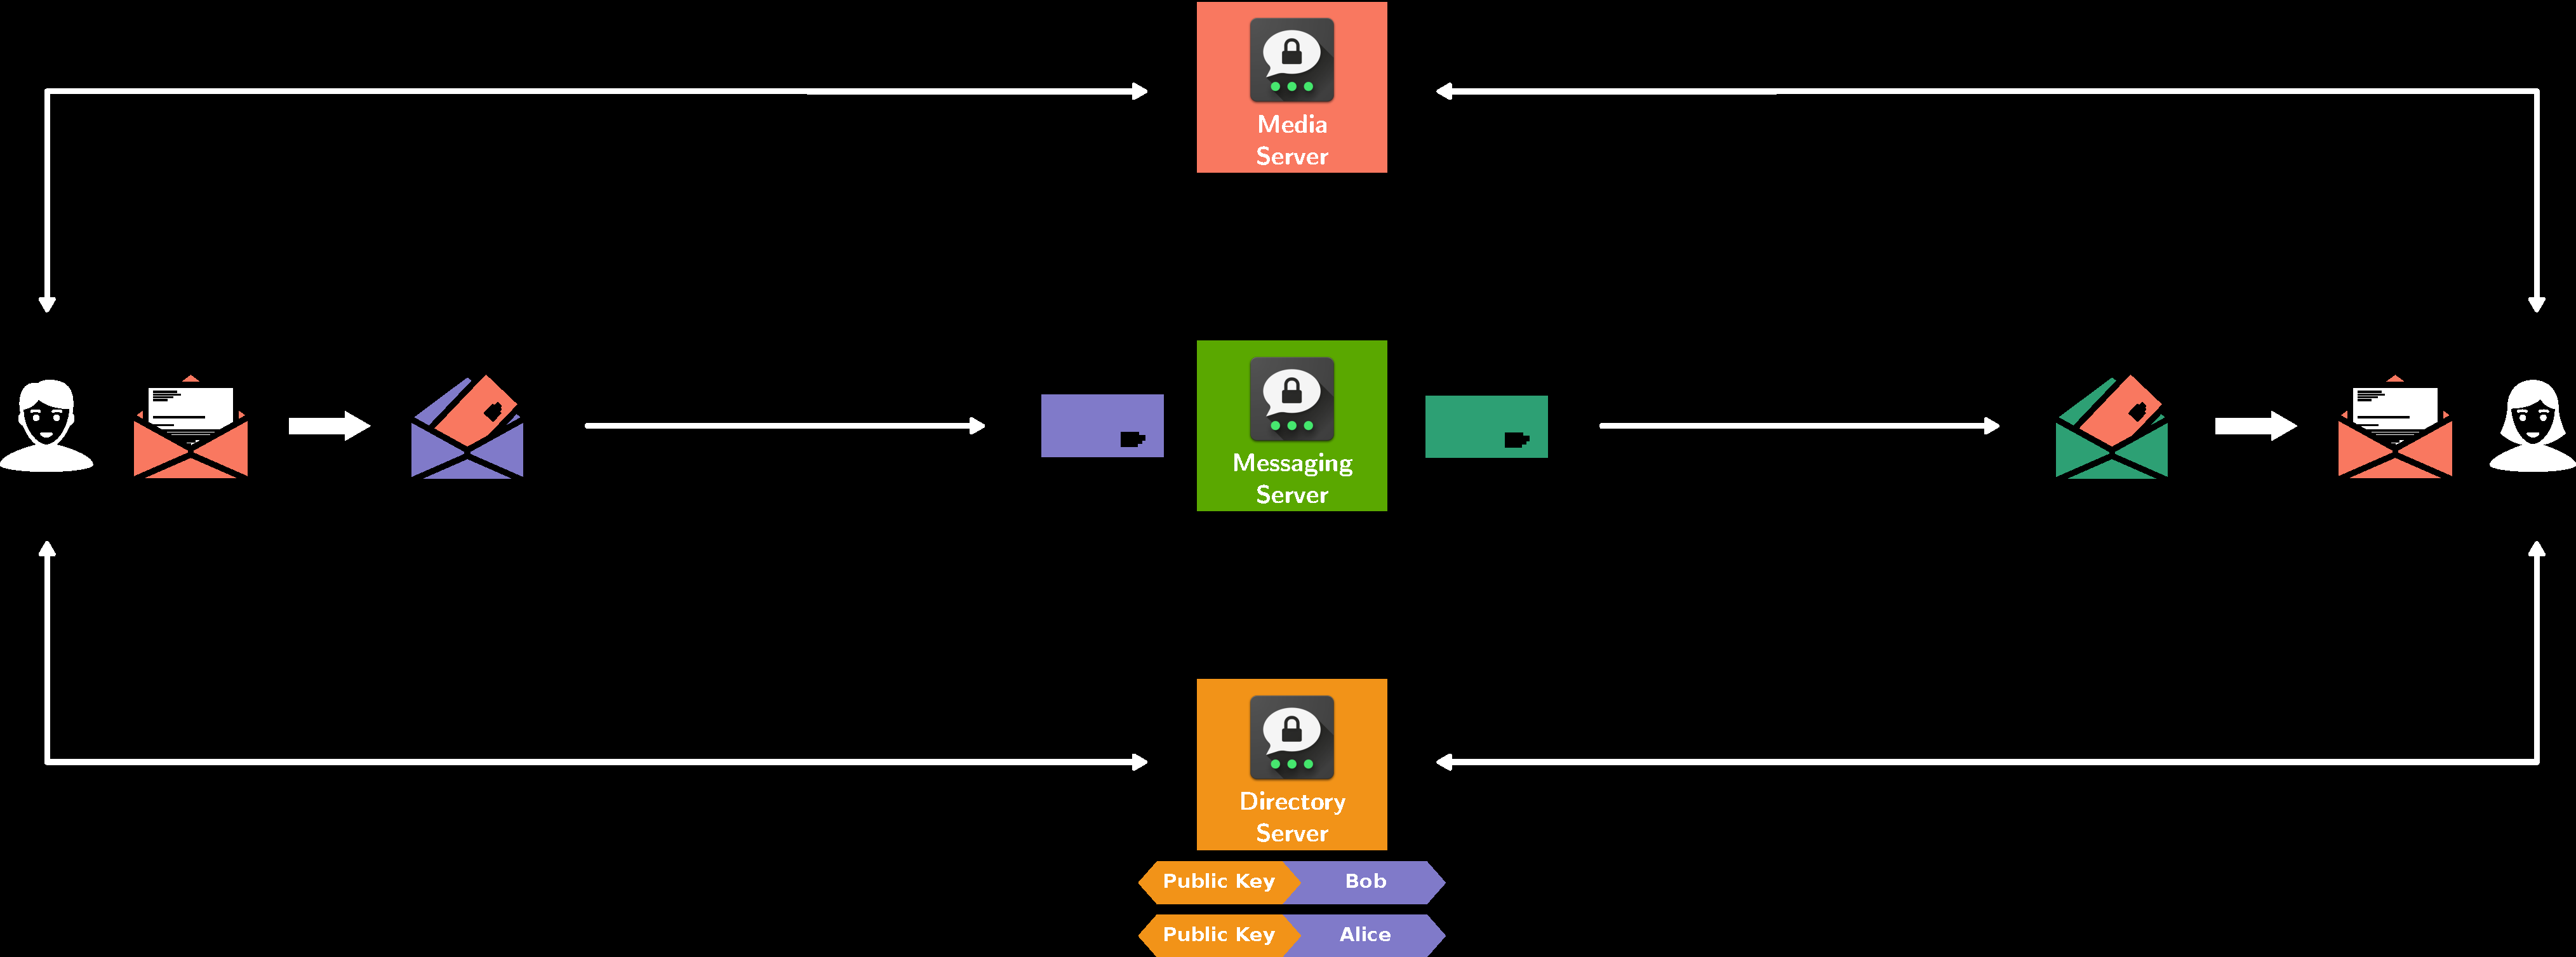
\includegraphics[width=\textwidth]{img/threema-architecture-overview.pdf}
	\pdfcomment{Coversation starts with Directory Server}
	\pdfcomment{Messaging server is the most essential}
	\pdfcomment{MediaServer is for transmission of big files, will e explained later}
\end{frame}

\begin{frame}
	\frametitle{Threema Fingerprints}
	\-\\[-.1em]
	\begin{columns}
		\begin{column}{.3\textwidth}
			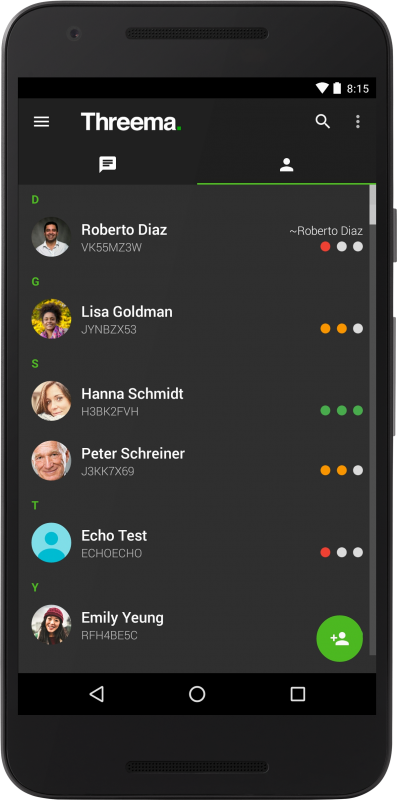
\includegraphics[height=.9\textheight]{img/android-nexus5x-2.6-us_en-dark-10-contacts-portrait-deviceart.png}
		\end{column}
		\begin{column}{.7\textwidth}
			Threema offers dedicated IDs		
			\begin{itemize}
				\item Users \alert{may} provider their phone number and email.
				\item If provided, phone number and email are used for identification with the directory server.
				\item If no additional data is provided, IDs can only be exchanged manually.
				\item In either case, manual verification using QR codes is encouraged.
				\item The app permanently tracks the verification status of each peer ID.
			\end{itemize}
		\end{column}
	\end{columns}
	\pdfcomment{Tackles the PKI problem explained earlier}
	\pdfcomment{Solution is pretty good. Reason why we chose 3ma}
	\pdfcomment{Less trust in Keys from Directory Server based on Threema ID}
	\pdfcomment{	more if based on phone number and email}
	\pdfcomment{	most if verified by qr}
\end{frame}

\begin{frame}
	\frametitle{NaCl and Threema}
	\-\\[2em]
	\begin{overlayarea}{\textwidth}{\textheight}
		\only<1>{%
			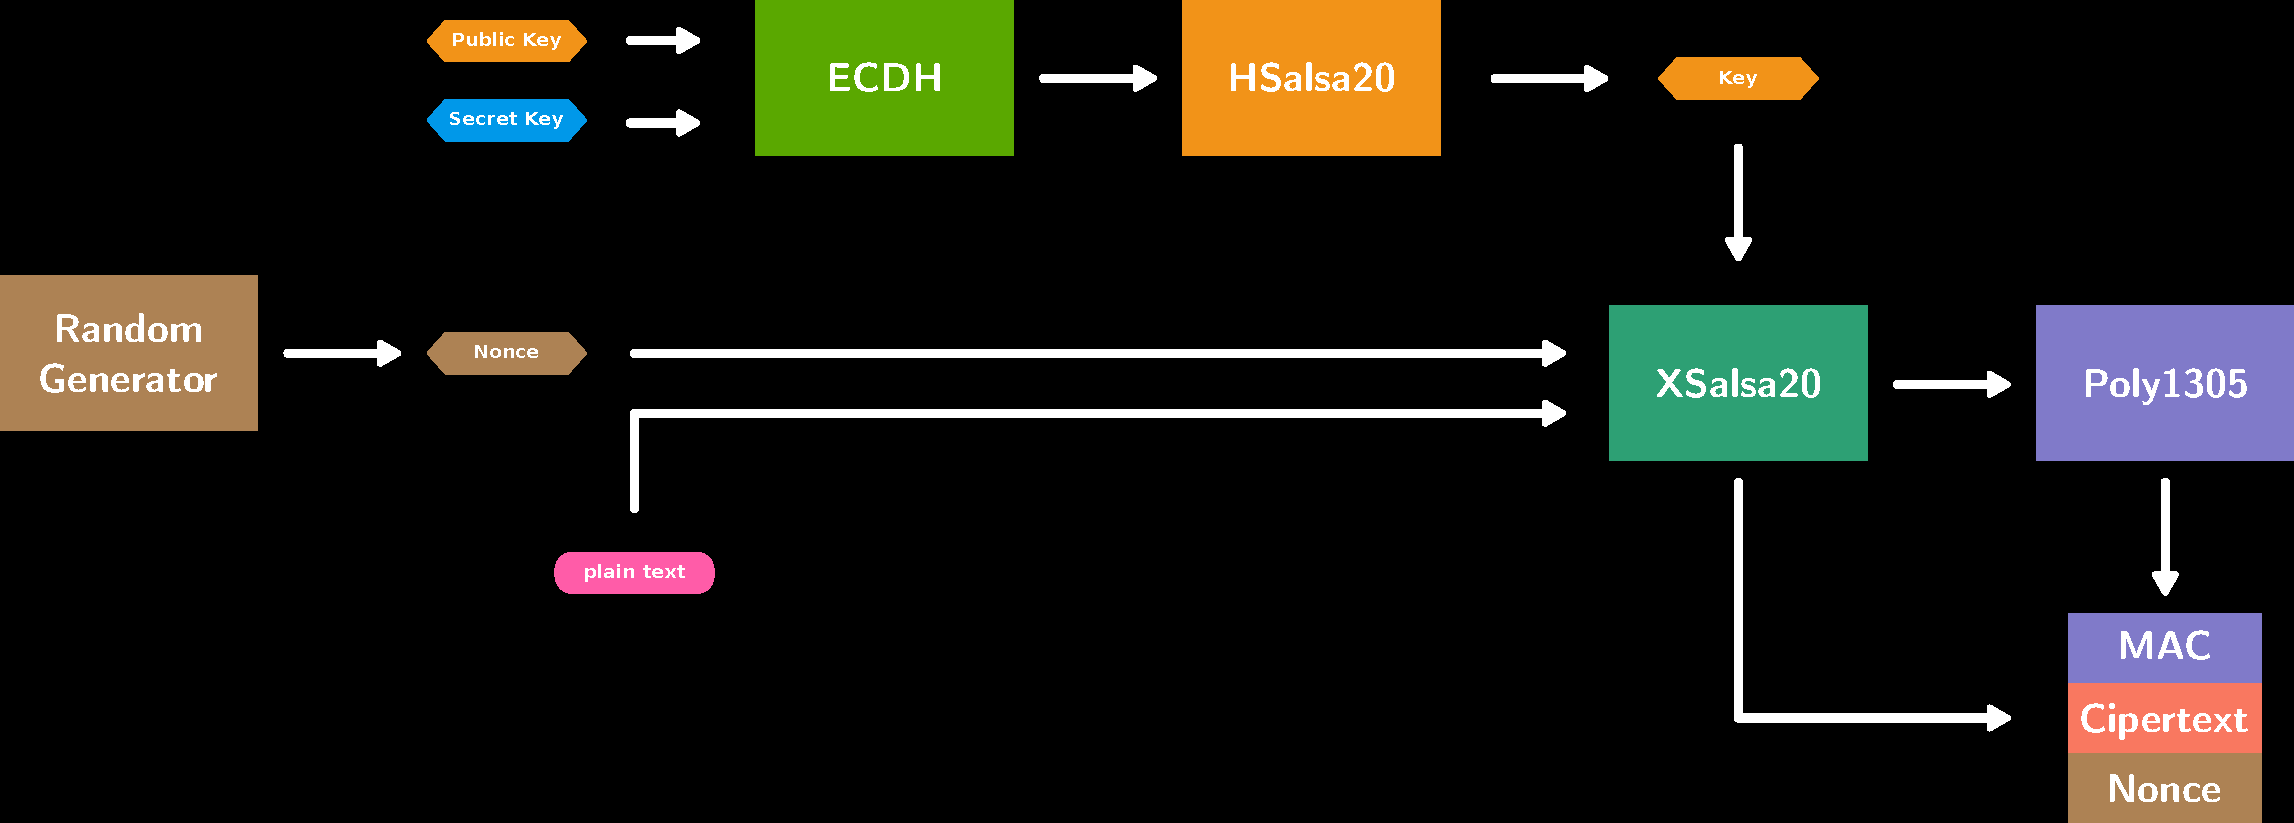
\includegraphics[width=\textwidth]{img/NaCl.pdf}
		}
		\only<2>{%
			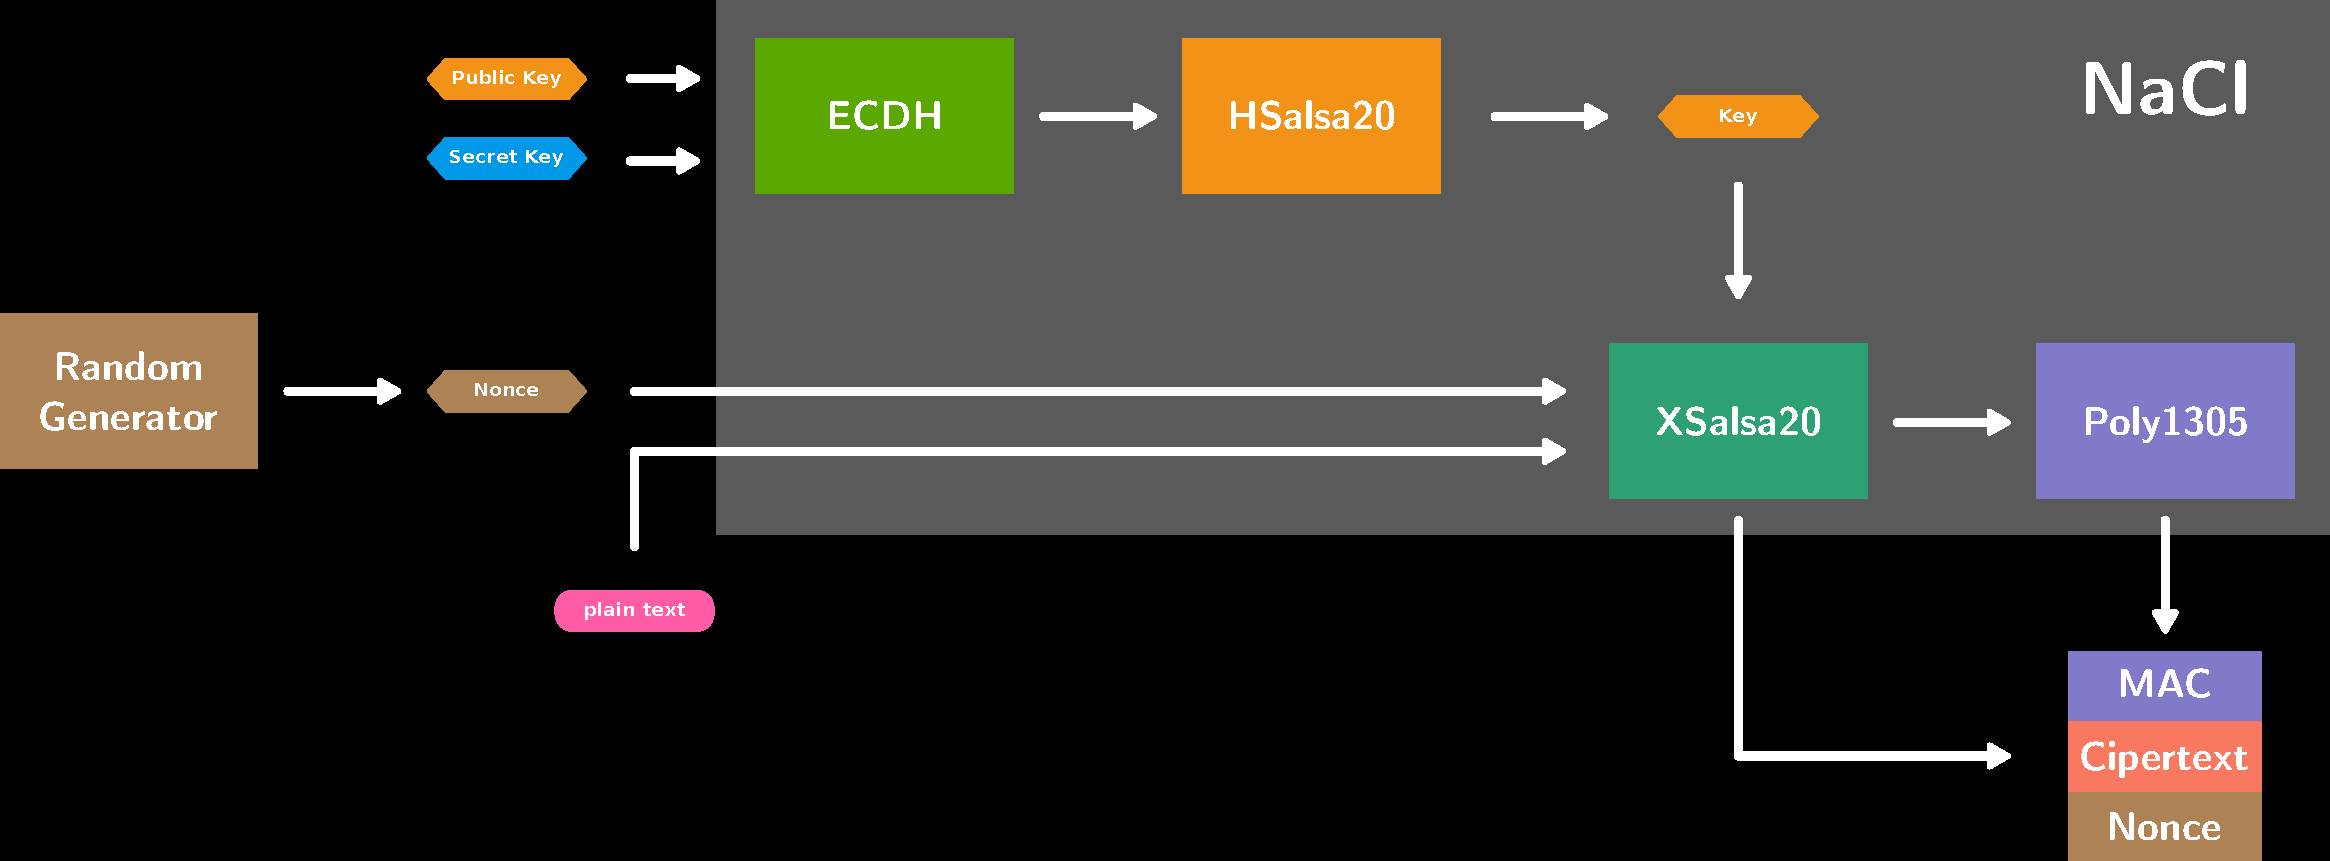
\includegraphics[width=\textwidth]{img/NaCl-highlight.pdf}
		}
	%\pdfcomment{NaCl exists and it works as roland explained in "autheticated encryption"}
	%\pdfcomment{3ma uses it}
	%\pdfcomment{c = crypto_box(msg,nonce,pk,sk)}
	\end{overlayarea}
	\pdfcomment{Salt gives us what is called 'authenticated encryption', which gives us authenticity, integrity and confidentiality}
\end{frame}


\begin{frame}[t]
	\frametitle{Threema's Handshake Between the App and the Messaging Server}
	\begin{overlayarea}{\textwidth}{\textheight}
		\begin{columns}
			\begin{column}[t]{.3\textwidth}
				\begin{overlayarea}{\textwidth}{\textheight}
					\only<1>{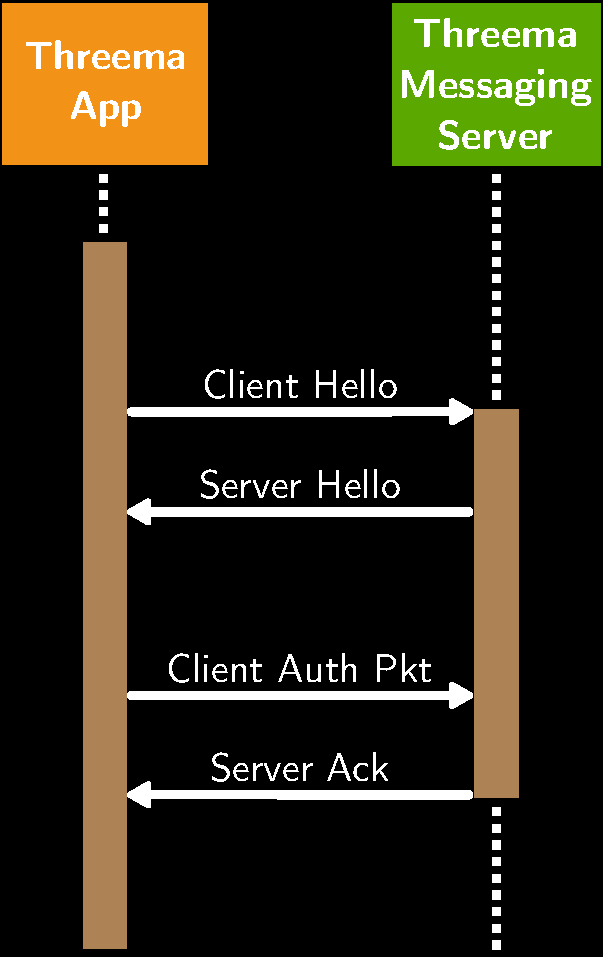
\includegraphics[width=\textwidth]{img/handshake.pdf}}	
					\only<2>{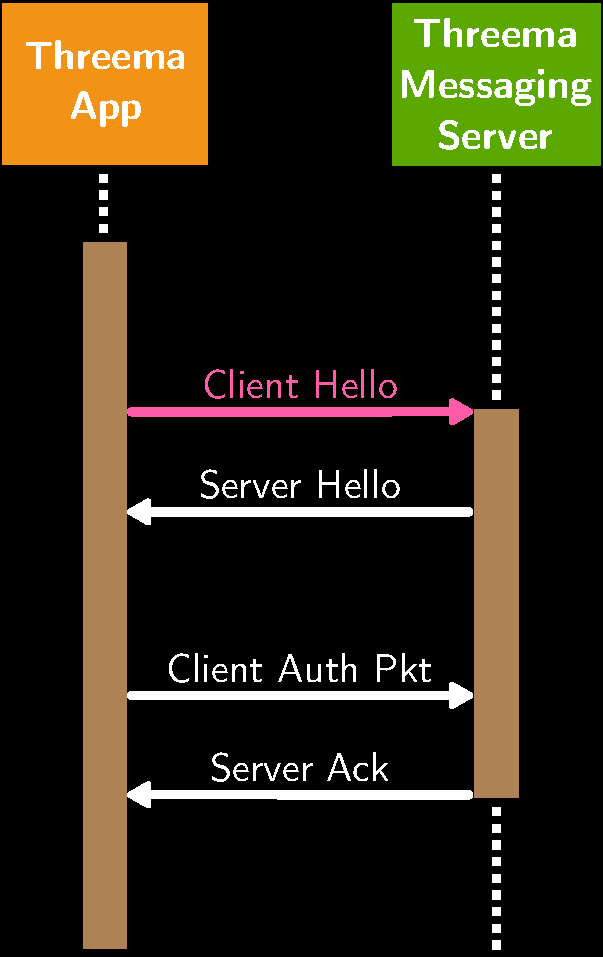
\includegraphics[width=\textwidth]{img/handshake-1.pdf}}	
					\only<3>{\includegraphics[width=\textwidth]{img/handshake-2.pdf}}	
					\only<4>{\includegraphics[width=\textwidth]{img/handshake-3.pdf}}	
					\only<5>{\includegraphics[width=\textwidth]{img/handshake-4.pdf}}	
				\end{overlayarea}
			\end{column}
			\begin{column}[t]{.01\textwidth}
			%padding
			\end{column}
			\begin{column}[t]{.69\textwidth}
				\begin{overlayarea}{\textwidth}{\textheight}
					\-\\%invisible line break
					\only<1>{%
						Exchange a set of \alert{ephemeral keys} and verify each others long term identity keys.
					}
					\only<2>{%
						{\large Client Hello Packet}\\[1ex]
						\includegraphics[page=11,clip,trim={.99cm 9cm 3.2cm 2.55cm},width=\textwidth]{out/messages.pdf}
						\begin{itemize}
							\item Client generates a \alert{ephemeral key} pair
							\item Client generates random nonce prefix
						\end{itemize}
					}	
					\only<3>{%
						{\large Server Hello Packet}\\[1ex]
						\includegraphics[page=11,clip,trim={.99cm 3.5cm 3.2cm 6.9cm},width=\textwidth]{out/messages.pdf}
						\begin{itemize}
							\item Server generates \alert{ephemeral key} pair
							\item Server generates random nonce
							\item Ciphertext encrypted with Server Nonce, Client Ephemeral Key and Server Long-Term Key
						\end{itemize}
						\pdfcomment{Ciphertext is is not readable by someone with clients LTK (forward sec).}
						\pdfcomment{Proves servers possesion of LTK}
					}	
					\only<4>{%
						{\large Client Authentication Packet}\\[1ex]
						\includegraphics[page=12,clip,trim={.99cm 10cm 3.2cm 1.5cm},width=\textwidth]{out/messages.pdf}
						\begin{itemize}
							\item Outer Encryption with \alert{ephemeral Keys}
							\item Ciphertext links clients \alert{ephemeral key} pair to it's long term key pair
						\end{itemize}
					}	
					\only<5>{%
						{\large Server Acknowledgement Packet}\\[1ex]
						\includegraphics[page=12,clip,trim={.99cm 7cm 3.2cm 6.2cm},width=\textwidth]{out/messages.pdf}
						\begin{itemize}
							\item Server comfirms everything worked fine by encrypting something with both \alert{ephemeral keys}
							\item We have established a forward secure channel between app and messaging server.
						\end{itemize}
					}	
				\end{overlayarea} \end{column}
		\end{columns}
	\end{overlayarea}
\end{frame}

\begin{frame}
	\frametitle{A 2-Layer Tunnel}
		\begin{center}\includegraphics[width=\textwidth]{img/2-layer-tunnel2.pdf}\end{center}
		\pdfcomment{Now we have explained all layers of the protocol. But what do we want to do with it?}
		\pdfcomment{We want to exchange messages. Our messages, as explained, are the inner channel}
		\pdfcomment{And that's what we will look at next}
\end{frame}

\begin{frame}[t]
	\frametitle{Threema Packet Format}
	\-\\[1em]
	\includegraphics[page=1,clip,trim={.99cm 8cm 3.2cm 1.8cm},width=\textwidth]{out/messages.pdf}
	\pdfcomment{Sender and recipient are on the 'envelope' as outlined earlier}
\end{frame}

\begin{frame}[t]
	\frametitle{Threema Text Messages}
	\-\\[1em]
	\includegraphics[page=3,clip,trim={.99cm 7.5cm 3.2cm 1.8cm},width=\textwidth]{out/messages.pdf}
\end{frame}

\begin{frame}[t]
	\frametitle{Threema Image Messages}
	\-\\[1em]
	\includegraphics[page=4,clip,trim={.99cm 7.5cm 3.2cm 1.8cm},width=\textwidth]{out/messages.pdf}
\end{frame}


\begin{frame}
	\frametitle{Sending an Image Message}
	\-\\[2em]
	\begin{overlayarea}{\textwidth}{\textheight}
		\only<1>{\includegraphics[width=\textwidth]{img/threema-architecture-1.pdf}}
		\only<2>{\includegraphics[width=\textwidth]{img/threema-architecture-2.pdf}}
		\only<3>{\includegraphics[width=\textwidth]{img/threema-architecture-3.pdf}}
		\only<4>{\includegraphics[width=\textwidth]{img/threema-architecture-4.pdf}}
		\only<5>{\includegraphics[width=\textwidth]{img/threema-architecture-5.pdf}}
	\end{overlayarea}
\end{frame}


% \begin{frame}
% 	\frametitle{Threema: Special Messages}
% 	\begin{itemize}
% 		\item Polls
% 		\item Images with Caption
% 			\begin{itemize}
% 				\item Case of caption leak found
% 			\end{itemize}
% 		\item Audio Messages
% 			\begin{itemize}
% 				\item Leak Android version
% 				\item Possible StageFright vector
% 			\end{itemize}
% 	\end{itemize}
% \end{frame}

% \begin{frame}
% 	\frametitle{Threema Audio Messages}
% 	\includegraphics[page=5,clip,trim={.99cm 7.5cm 3.2cm 1.8cm},width=\textwidth]{out/messages.pdf}
% \end{frame}

% \begin{frame}
% 	\frametitle{Threema Audio Messages -- Notes}
% 	\begin{itemize}
% 		\item Audio length is lost on forwarding
% 	\end{itemize}
% \end{frame}

\begin{frame}
	\frametitle{Recap}
	Basic messaging functionality achieved.
\end{frame}

\begin{frame}
	\frametitle{Group Messages}
	\-\\[2em]
	\begin{overlayarea}{\textwidth}{\textheight}
		\only<1>{%
			\includegraphics[page=6,clip,trim={.99cm 7.5cm 3.2cm 1.8cm},width=\textwidth]{out/messages.pdf}
			\pdfcomment{Group IDs aren't unique. They are created locally and only work together with the group creator's ID}
			\pdfcomment{The structure of group messages makes it impossible for Threema to introduce multiple group administrators on a protocol level without breaking compatibility to older clients.}
		}
	\end{overlayarea}
\end{frame}

\begin{frame}
	\frametitle{Group Management Messages}
	\-\\[2em]
	\begin{overlayarea}{\textwidth}{\textheight}
		\only<1>{%
			Group creation message\\[1em]
			\includegraphics[page=14,clip,trim={.99cm 7.5cm 3.2cm 1.8cm},width=\textwidth]{out/messages.pdf}

		}
		\only<2>{%
			Group rename message\\[1em]
			\includegraphics[page=15,clip,trim={.99cm 7.5cm 3.2cm 1.8cm},width=\textwidth]{out/messages.pdf}

		}
	\end{overlayarea}
\end{frame}


\begin{frame}[t]
	\frametitle{Implementation of Addon Features}

	\only<1>{%
		Captions in Image Messages\\[2em]

		\begin{center}
			\includegraphics[width=.6\textwidth]{img/exif.pdf}
		\end{center}
		\pdfcomment{Captions are stored in Exif.Photo.UserComment and Exif.Image.Artist}
	}
	\only<2>{%
		Quoted Messages\\[1em]
		\begin{center}
			\includegraphics[page=16,clip,trim={.99cm 7.5cm 7.2cm 1.8cm},width=.7\textwidth]{out/messages.pdf}\\[1em]
			\includegraphics[width=.25\textwidth]{img/quote.png}
		\end{center}
		\pdfcomment{Has to be a Threema ID, not a nickname}
	}
		
\end{frame}



\begin{frame}
	\frametitle{The Devil's in the Detail}
	Sammlung kleinerer Dinge, die uns aufgefallen sind
	\begin{itemize}
		\item Media messages could be StageFright attack vectors
		\item The protocol implementation looks sound to us but the message design prevents feature upgrades on the protocol (not text-protocol) level
		\item Retention policies for uploaded Blobs
	\end{itemize}
\end{frame}


%\begin{frame}
%	\frametitle{Threema - Notes and Open Questions}
%	Notes:
%	\begin{itemize}
%		\item PFS only on transport layer (attacker sniffing packets from the outside will not learn contents after private key acquisition)
%	\end{itemize}
%	Q:
%	\begin{itemize}
%		\item How often is the handshake performed?
%	\end{itemize}
%\end{frame}

%\section{Case Study - Signal}

%\begin{frame}
%	\frametitle{Signal Forward and Future Secrecy}
%	\begin{itemize}
%		\item If you want forward secrecy, you need to use asymmetric crypto and dispose of your keys as often as possible
%		\item To do that you need to perform a new handshake frequently
%		\item Since it is not always given that both parties are online for that handshake, the good people of Whispersystems have come up with this:
%			\begin{enumerate}
%				\item Both parties upload a bunch of keys to the server. Those are signed identity keys as we've seen previously and a large number of \alert{prekeys}
%				\item Using a prekey, any party can perform their part of the handshake offline and end up with a new session key to use 
%				\item These session keys are renewed by \alert{ratcheting} with each message transfer
%			\end{enumerate}
%	\end{itemize}
%\end{frame}
%
%\begin{frame}
%	\frametitle{Signal - Notes}
%	\begin{itemize}
%		\item Server-side cached short-term keys (\alert{prekeys}) fetched by sender
%		\item Pairwise long-lived symmetric secret key between participants
%		\item Multiple messages without answer $\rightarrow$ perform KDF on \alert{chaining key}
%		\item ECDH: Curve25519, AES-CTR (no padding), AES-CBC (PKCS7 padding)
%		\item HMAC-SHA256 for integrity
%		\item Future secrecy only if private keys are not leaked (duh!). Since private keys go into new shared keys during ratcheting, the attacker lacks material to compromise next key after obtaining current one.
%		\item Since shared keys are only deleted after messages are received, there is a window in which keys could be compromised before reception. 
%		\item Deniability is always a theoretical claim as long as a transmission server has the ability to log messages, their senders and recipients.
%
%	\end{itemize}
%\end{frame}

%\section{Reverse-Engineering Threema}

%\begin{frame}
%	\frametitle{Enter Threema}
%	Threema
%	\begin{itemize}
%		\item Gained popularity in Germany after Facebook purchased WhatsApp
%		\item All promise -- no proof; first openly contemplating to OSS the code, later backing away from that statement
%		\item Interest in its inner workings
%	\end{itemize}
%
%	Quick Shoutouts
%	\begin{itemize}
%		\item Jan Ahrens for releasing his findings about the handshake before we did
%		\item OpenMittsu for releasing the first working OSS client
%	\end{itemize}
%	
%\end{frame}

%\begin{frame}
%	\frametitle{Reverse-Engineering -- What to look for?}
%	\begin{itemize}
%		\item Test for common pitfalls in implementation
%			\begin{itemize}
%				\item Handling of TLS
%				\item Handling of keys and nonces
%				\item NaCl implementation errors
%				\item Uncommon data leaks
%				\item Bugs
%				\item \ldots?
%			\end{itemize}
%		\item Find out how protocol is designed
%			\begin{enumerate}
%				\item Understand handshakes
%				\item Understand protocol
%				\item decipher messages
%			\end{enumerate}
%	\end{itemize}
%	\alert{Positive side-note}: Threema had released a security white paper early on
%\end{frame}

\begin{frame}
	\frametitle{Our Library}

	Our reverse-engineering efforts led to a re-implementation of Threema's API.

	
\end{frame}

\begin{frame}[plain,t]
	\frametitle{Done!}
	\-\\[.5em]
	{\Huge\bfseries Thank You!} \\[2em]
	\begin{columns}[t]
		\begin{column}[t]{.3\textwidth}
			\textbf{Roland Schilling}\\[.8ex]
			\begin{tabular}{rl}
				\parbox[c]{1ex}{\iconmail{15}}    & \scriptsize{\url{schilling@tuhh.de}}\\
				\parbox[c]{1ex}{\icontwitter{15}} & \scriptsize{\url{@NerdingByDoing}}\\
			\end{tabular}
		\end{column}
		\begin{column}[t]{.635\textwidth}
			\textbf{Frieder Steinmetz\phantom{g}}\\[.8ex] %phantom-g because \\ doesn't align to baseline
			\begin{tabular}{rl}
				\parbox[c]{1ex}{\iconmail{15}}    & \scriptsize{\url{frieder.steinmetz@tuhh.de}}\\
				\parbox[c]{1ex}{\icontwitter{15}} & \scriptsize{\url{@twillnix}}\\
			\end{tabular}
		\end{column}
	\end{columns}
	\alert{\rule{.75\textwidth}{1pt}}\\[1.5em]
	\tiny
	\begin{tabular}{@{}ll}
		Beamer Theme: & \alert{\href{https://github.com/matze/mtheme}{Metropolis}} by Matthias volgelsang\\
		Color Theme: & \alert{\href{https://github.com/rchurchley/beamercolortheme-owl}{Owl}} by Ross Chirchley \\
		Icons: & \alert{\href{https://thenounproject.com/mockturtle/collection/big/}{The BIG collection}} by Sergey Demushkin\\
		 & \alert{\href{http://zurb.com/playground/foundation-icon-fonts-3}{Foundation Icon Fonts 3}} by ZURB\\
		 \multicolumn{2}{@{}l}{NaCl slide was adapted from a figure in Threema's \alert{\href{https://threema.ch/press-files/2_documentation/cryptography_whitepaper.pdf}{Cryptography Whitepaper}}}\\
		 \multicolumn{2}{@{}l}{Threema Screenshots taken from the \alert{\href{https://threema.ch/en/press}{Threema press package}}}\\
	\end{tabular}\\[2em]
	Thanks to \alert{Jan Ahrens} and \alert{Philipp Berger} -- their work has made ours somewhat easier\\
	Thanks to \alert{Maximilian Köstler} for his initial work on Threema

\end{frame}

\appendix

%\section*{Appendix}

\begin{frame}
	\frametitle{Appendix}

	\forloop{i}{1}{\value{i} < \value{messagepages}}{%
		\only<\value{i}>{%
			\centering%
			\includegraphics[width=\textwidth,page=\value{i}]{out/messages.pdf}%
		}%
	}
\end{frame}

\end{document}

% vim: spelllang=en spell
